\documentclass[../main.tex]{subfiles}
\begin{document}

\chapter*{Preface}
\addcontentsline{toc}{section}{Preface}

This book is intended for an advanced undergraduate or a first-year graduate course in numerical linear algebra, a very important topic for engineers and scientists. Many of the numerical methods used to solve engineering and science problems have linear algebra as an important component. Examples include spline interpolation, estimation using least squares, and the solution of ordinary and partial differential equations. It has been said that, next to calculus, linear algebra is the most important component in engineering problem solving. In computer science, linear algebra is a critical as well. The Google matrix is an example, as is computer graphics where matrices are used for rotation, projection, rescaling, and translation. Applications to engineering and science are provided throughout the book.

Two important problems in a customary applied linear algebra course are the solution of general linear algebraic systems $Ax = b$, where $A$ is an $m \times n$ matrix, and the computation of eigenvalues and their associated eigenvectors. If the system is square $(m = n)$ and nonsingular, the student is taught how to find a solution to $Ax = b$ using Cramer’s Rule, Gaussian elimination and multiplication by the inverse. In many areas of application, such as statistics and signal processing, $A$ is square and singular or $m \neq n$. In these situations, the transformation to reduced row echelon form produces no solution or infinitely many, and this is just fine in a theoretical sense, but is not helpful for obtaining a useful solution. Eigenvalues are often discussed late in the course, and the student learns to compute eigenvalues by finding the roots of the characteristic polynomial, never done in practice.

A study of numerical linear algebra is different from a study of linear algebra. The problem is that many of the theoretical linear algebra methods are not practical for use with a computer. To be used on a computer, an algorithm, a method for solving a problem step by step in a finite amount of time, must be developed that deals with the advantages and problems of using a computer. Any such algorithm must be efficient and not use too much computer memory. For instance, Cramer’s Rule is not practical for matrices of size $4 \times 4$ or greater, since it performs far to many operations. Since a digital computer performs arithmetic in binary with a fixed number of digits, errors occur when entering data and performing computations. For instance, $1/3$ cannot be represented exactly in binary, and its binary representation must be approximated. In addition, computation using the operations of addition, subtraction, multiplication, and division rarely can be done exactly, resulting in errors. An algorithm must behave properly in the presence of these inevitable errors; in other words, small errors during computation should produce small errors in the output. For example, the use of Gaussian elimination to solve an $n \times n$ linear system should use a method known as partial pivoting to control errors. When the matrix $A$ is $m \times n$, $m \neq  n$, a solution must be obtained in the sense of least-squares, and the efficient and implementation of least-squares presents challenges. The eigenvalue problem is of primary importance in engineering and science. In practice, eigenvalues are not found by finding the roots of a polynomial, since polynomial root finding is very prone to error. Algorithms have been developed for accurate solution of the eigenvalue problem on a computer.

In the book, algorithms are stated using pseudocode, and MATLAB is the vehicle used for algorithm implementation. MATLAB does a superb job of dealing with numeric computation and is used in most engineering programs. Accompanying the text is a library of MATLAB functions and programs, named NLALIB, that implements most of the algorithms discussed in the book. Many examples in the book include computations using MATLAB, as do many exercises. In some cases, a problem will require the student to write a function or program using the MATLAB programming language. If the student is not familiar with MATLAB or needs a refresher, the MathWorks Web site www.mathworks.com provides access to tutorials. There are also many free online tutorials.

If the reader does not have access to MATLAB, it is possible to use GNU Octave, a system primarily intended for numerical computations. The Octave language is quite similar to MATLAB so that most programs are easily portable.

This book is novel, in that there is no assumption the student has had a course in linear algebra. Engineering students who have completed the usual mathematics sequence, including ordinary differential equations, are well prepared. The prerequisites for a computer science student should include at least two semesters of calculus and a course in discrete mathematics. Chapters $1 \_ 6$ supply an introduction to the the basics of linear algebra. A thorough knowledge of these chapters prepares the student very well for the remainder of the book. If the student has had a course in applied or theoretical linear algebra, these chapters can be used for a quick review.

Throughout the book, proofs are provided for most of the major results. In proofs, the author has made an effort to be clear, to the point of including more detail than normally provided in similar books. It is left to the instructor to determine how much emphasis should be given to the proofs.

The exercises include routine pencil and paper computations. Exercises of this type force the student to better understand the workings of an algorithm. There are some exercises involving proofs. Hints are provided if a proof will be challenging for most students. In the problems for each chapter, there are exercises to be done using MATLAB.

\subsection*{TOPICS}
Chapters 1-6 provide coverage of applied linear algebra sufficient for reading the remainder of the book.

\subsection*{Chapter 1: Matrices}
The chapter introduces matrix arithmetic and the very important topic of linear transformations. Rotation matrices provide an interesting and useful example of linear transformations. After discussing matrix powers, the concept of the matrix inverse and transpose concludes the chapter.

\subsection*{Chapter 2: Linear Equations}
This chapter introduces Gaussian elimination for the solution of linear systems $Ax = b$ and for the computation of the matrix inverse. The chapter also introduces the relationship between the matrix inverse and the solution to a linear homogeneous equation. Two applications involving a truss and an electrical circuit conclude the chapter.

\subsection*{Chapter 3: Subspaces}
This chapter is, by its very nature, somewhat abstract. It introduces the concepts of subspaces, linear independence, basis, matrix rank, range, and null space. Although the chapter may challenge some readers, the concepts are essential for understanding many topics in the book, and it should be covered thoroughly.

\subsection*{Chapter 4: Determinants}
Although the determinant is rarely computed in practice, it is often used in proofs of important results. The chapter introduces the determinant and its computation using expansion by minors and by row elimination. The chapter ends with an interesting application of the determinant to text encryption.

\subsection*{Chapter 5: Eigenvalues and Eigenvectors}
This is a very important chapter, and its results are used throughout the book. After defining the eigenvalue and an associated eigenvector, the chapter develops some of their most important properties, including their use in matrix diagonalization. The chapter concludes with an application to the solution of systems of ordinary differential equations and the problem of ranking items using eigenvectors.

\subsection*{Chapter 6: Orthogonal Vectors and Matrices}
This chapter introduces the inner product and its association with orthogonal matrices. Orthogonal matrices play an extremely important role in matrix factorization. The L2 inner product of functions is briefly introduced to emphasize the general concept of an inner product.

\subsection*{Chapter 7: Vector and Matrix Norms}
The study of numerical linear algebra begins with this chapter. The analysis of methods in numerical linear algebra relies heavily on the concept of vector and matrix norms. This chapter develops the 2-norm, the 1-norm, and the infinity norm for vectors. A development of matrix norms follows, the most important being matrix norms associated with a vector norm, called subordinate norms. The infinity and 1-norms are easy to compute, but the connection between their computation and the mathematical definition of the a matrix norm is somewhat complex. A MATLAB program motivates the process for the computation of the infinity norm, and the chapter contains a complete proof verifying the algorithm for computing the infinity norm. The 2-norm is the most useful matrix norm and by far the most difficult to compute. After motivating the computation process with a MATLAB program, the chapter provides a proof that the 2-norm is the square root of the largest singular value of the matrix and develops properties of the matrix 2-norm.

\subsection*{Chapter 8: Floating Point Arithmetic}
The chapter presents the representation of integer and floating point data in a computer, discusses the concepts of overflow and underflow, and explains why roundoff errors occur that cannot be avoided. There is a careful discussion concerning the concepts of absolute and relative error measurement and why relative error is normally used. The chapter presents a mathematical analysis of floating point errors for addition and states results for other operations. The chapter concludes with a discussion of situations where a careful choice of algorithm can minimize errors. This chapter is critical for understanding the remaining chapters. The only content that can be reasonably omitted is the mathematical discussion of floating point
errors.

\subsection*{Chapter 9: Algorithms}
The algorithms in the book are presented using pseudocode, and the pseudocode is quite complete. It is intended that in most cases the conversion between pseudocode and MATLAB should not be difficult. The chapter introduces the concept of algorithm efficiency by computing the the number of floating point operations, called the flop count, or representing it using big-O notation. The presentation of algorithms for matrix multiplication, the solution to upper and lower triangular systems, and the Thomas algorithm for the solution of a tridiagonal system are the primary examples. Included is a brief discussion of block matrices and basic block matrix operations.

\subsection*{Chapter 10: Conditioning of Problems and the Stability of Algorithms}
The chapter introduces the concept of stability and the conditioning. An algorithm is unstable if small changes in the data can cause large changes in the result of the computation. An algorithm may be stable, but the data supplied to the algorithm can be ill-conditioned. For instance, some matrices are very sensitive to errors during Gaussian elimination. After discussing examples and introducing some elementary perturbation analysis using backward and forward error, the chapter develops the condition number of a matrix and its properties. The condition number of a matrix plays an important role as we develop algorithms in the remainder of the book. This material is at the heart of numerical linear algebra and should be covered at least intuitively. There are a number of problems involving numerical experiments, and some of these should be done in order to appreciate the issues involved.

\subsection*{Chapter 11: Gaussian Elimination and the LU Factorization}
This chapter introduces the LU decomposition of a square matrix. The LU decomposition uses Gaussian elimination, but is not a satisfactory algorithm without using partial pivoting to minimize errors. The LU decomposition properly computed can be used to solve systems of the form $Ax_{i} = b_{i}, 1 \leq i \leq k$. The somewhat expensive Gaussian elimination algorithm need be used only once. After its computation, many solutions $\{x_{i}\}$ are quickly found using forward and back substitution.

\subsection*{Chapter 12: Linear Systems Applications}
Four applications that involve linear systems comprise this chapter. A discussion of Fourier series introduces the concept of an infinite dimensional vector space and provides an application for the $L^{2}$ inner product introduced in Chapter 6. A second application involves finite difference approximations for the heat equation. Finite difference techniques are important when approximating the solution to boundary value problems for ordinary and partial differential equations. Chapter 16 discusses least-squares problems. As a tune-up for this chapter, the third application develops approximation by polynomial least-squares. The last application is a discussion of cubic spline interpolation. Using this process, a series of cubic polynomials are fitted between each pair of data points over an interval $a \leq  x \leq  b$, with the requirement that the curve obtained be twice differentiable. These cubic splines can then be used to very accurately estimate the data at other points in the interval. The
computation of cubic splines involves the solution of a tridiagonal system of equations, and the Thomas algorithm presented in Chapter 9 works very well.

\subsection*{Chapter 13: Important Special Systems}
Numerical linear algebra is all about computing solutions to problems accurately and efficiently. As a result, algorithms must be developed that take advantage of a special structure or properties of a matrix. This chapter discusses the factorization of a tridiagonal matrix and the Cholesky factorization of a symmetric positive definite matrix. In both cases, the matrix factorization leads to more efficient means of solving a linear system having a coefficient matrix of one of these types.

\subsection*{Chapter 14: Gram-Schmidt Orthonormalization}
The Gram-Schmidt algorithm for computing an orthonormal basis is time-honored and important. It becomes critical in the development of algorithms such as the singular value and Arnoldi decompositions. The chapter carefully develops the QR decomposition using Gram-Schmidt. Although the decomposition is not normally done this way, it serves to demonstrate that this extremely important tool exists. As a result, the MATLAB algorithm qr can be used with some understanding until efficient methods for the QR decomposition are explained.

\subsection*{Chapter 15: The Singular Value Decomposition}
The singular value decomposition (SVD) is perhaps the most important result in numerical linear algebra. Its uses are many, including providing a method for estimating matrix rank and the solution of least-squares problems. This chapter proves the SVD theorem and provides applications. Perhaps the most interesting application is the use of the SVD in image compression. Practical algorithms for the computation of the SVD are complex, and are left to Chapter 23.

\subsection*{Chapter 16: Least Squares Problems}
Approximation using least-squares has important applications in statistics and many other areas. For instance, data collected by sensor networks is often analyzed using least-squares in order to approximate events taking place. Least-squares problems arise when the data requires the solution to an $m \times  n$ system $Ax = b$ , where $m \neq n$. Normally, there is no solution $ \bar{x}$ such that $A \bar{x} = b$ , or there are infinitely many solutions, so we seek a solution that minimizes the Euclidean norm of $Ax - b$. Least-squares provides an excellent application for the QR factorization and the SVD.
\subsection*{Chapter 17: Implementing the QR Factorization}
The QR factorization using the Gram-Schmidt process was developed in Chapter 14. This chapter presents two other approaches to the factorization, the use of Givens rotations and Householder reflections. In each case, the algorithm is more stable than Gram-Schmidt. Also, we will have occasion to use Givens rotations and Householder reflections for other purposes, such as the computation of eigenvalues. If a detailed presentation is not required, these ideas have a nice geometrical interpretation.
\subsection*{Chapter 18: The Algebraic Eigenvalue Problem}
The applications of the eigenvalue problem are vast. The chapter begins by presenting three applications, a problem in vibration and resonance, the Leslie model in population biology, and the buckling of a column. The accurate computation of eigenvalues and their associated eigenvectors is difficult. The power and inverse power methods are developed for computing the largest and smallest eigenvalues of a matrix. These methods are important but have limited use. The chapter discusses the QR iteration for the computation of all the eigenvalues and their associated eigenvectors of a real matrix whose eigenvaluesare distinct. The development is detailed and includes the use of the shifted Hessenberg QR iteration. The chapter also develops the computation of eigenvectors using the Hessenberg inverse iteration. The method used in most professional implementations is the implicit QR iteration, also known as the Francis iteration. The chapter develops the algorithm for the computation of both the real and complex eigenvalues of a real matrix.

\subsection*{Chapter 19: The Symmetric Eigenvalue Problem}
If a matrix is symmetric, an algorithm can exploit its symmetry and compute eigenvalues faster and more accurately. Fortunately, many very important problems in engineering and science involve symmetric matrices. The chapter develops five methods for the computation of eigenvalues and their associated eigenvectors, the Jacobi method, the symmetric QR iteration method, the Francis algorithm, the bisection method, and the divide and conquer method.
\subsection*{Chapter 20: Basic Iterative Methods}
Iterative methods are used for the solution of large, sparse, systems, since ordinary Gaussian elimination operations will destroy the sparse structure of the matrix. This chapter presents the classical Jacobi, Gauss-Seidel, and SOR methods, along with discussion of convergence. The chapter concludes with the application of iterative methods to the solution of the two-dimensional Poisson equation.

\subsection*{Chapter 21: Krylov Subspace Methods}
This is a capstone chapter, and should be covered, at least in part, in any numerical linear algebra course. The conjugate gradient method (CG) for the solution of large, sparse symmetric positive definite systems is presented. This method is one of the jewels of numerical linear algebra and has revolutionized the solution of many very large problems. The presentation motivates the algorithm and provides mathematical details that explain why it works. The conjugate gradient method is a Krylov subspace method, although the book does not develop it using this approach. However, the next algorithm presented is the general minimum residual method (GMRES) for the iterative solution of large, sparse, general matrices, and it is approached as a Krylov subspace method. The Krylov subspace-based minimum residual (MINRES) method for the solution of large, sparse, symmetric, non-positive definite matrices is the last method presented. If a matrix is ill-conditioned, CG, GMRES, and MINRES do not perform well. The solution is to precondition the system before applying an iterative method. The chapter presents preconditioning techniques for CG and GMRES. After presenting a chart detailing approaches to large, sparse problems, the chapter concludes with another approach to the Poisson equation and a discussion of the biharmonic equation that is one of the most important equations in applied mechanics.

\subsection*{Chapter 22: Large Sparse Eigenvalue Problems}
The chapter discusses the use of the Arnoldi and Lanczos processes to find a few eigenvalues of large, sparse matrices. Two approaches are discussed, explicit and implicit restarting. The mathematics behind the performance of these methods is beyond the scope of the text, but the algorithms are presented and MATLAB implementations provided. Various exercises test the methods and clearly demonstrate the challenge of this problem.

\subsection*{Chapter 23: Computing the Singular Value Decomposition}
The chapter develops two methods for computing the SVD, the one-sided Jacobi method, and the Demmel and Kahan zero-shift QR downward sweep algorithm. Developing the two methods requires a knowledge of many results from earlier chapters.

\subsection*{Appendices A, B, and C}
Appendix A provides a discussion of complex numbers so that a reader unfamiliar with the topic will be able to acquire the knowledge necessary when the book uses basic results from the theory of complex numbers. Appendix B presents a brief discussion of mathematical induction, and Appendix C presents an overview of Chebyshev polynomials. Although these polynomials are not used within any proof in the book, they are referenced in theorems whose proofs are provided by other
sources.

\subsection*{INTENDED AUDIENCE}
Numerical linear algebra is often a final chapter in a standard linear algebra text, and yet is of paramount importance for engineers and scientists. The book covers many of the most important topics in numerical linear algebra, but is not intended to be encyclopedic. However, there are many references to material not covered in the book. Also, it is the author’s hope that the material is more accessible as a first course than existing books, and that the first six chapters provide material sufficient for the book to be used without a previous course in applied linear algebra. The book is also is very useful for self-study and can serve as a reference for engineers and scientists. It can also serve as an entry point to more advanced books, such as James Demmel’s book \cite{ref1}  or the exhaustive presentation of the topic by Golub and Van Loan \cite{ref2} .

\subsection*{WAYS TO USE THE BOOK}
The instructor will need to decide how much theory should be covered; namely, how much emphasis will be placed on understanding the proofs and doing problems involving proofs. If the students are not experienced with proofs, one approach is to explain methods and theorems as intuitively as possible, supporting the discussion with numerical examples in class, and having the students do numerous numerical exercises both in class and in assignments. For instance, using Jacobi rotations to compute the eigenvalues of a real symmetric matrix is easily explained using simple diagrams and running a MATLAB program included with the software distribution graphically demonstrates how the method performs a reduction to a diagonal matrix. This approach works well with engineering students who have little or no experience with theorems and proofs. They will learn how to solve problems, large and small, using the appropriate methods.

If the audience consists of students who are mathematics majors or who have significant mathematical training, then some proofs should be covered and assignments should include proofs. Some of these exercises include hints to get the student started. The author believes that for a student to stare at the hypothesis and conclusion only to give up in frustration makes no sense, when a simple hint will kick start the process.

Of course, the amount of material that the instructor can cover depends on the background of the students. Mathematics majors will likely have taken a theoretical or applied linear algebra course. After optionally reviewing the material in Chapters 1-6 the study of numerical linear algebra can begin. The following is a list of suggestions for various chapters that outlines material that can be omitted, covered lightly, or must be covered.

\begin{itemize}[noitemsep]
	
	\item  In Chapter 7, proofs that justify methods for computing matrix norms can be omitted, but MATLAB programs that motivate the methods should be discussed.

	\item Chapter 8 is essential to an understanding of numerical linear algebra. It presents storage formats for integers and floating point numbers and shows why the finite precision arithmetic used by a computer leads to roundoff error. Some examples are provided that show how rearranging the order of computation can help to reduce error.
	
	\item Chapter 10 that discusses the stability and conditioning of algorithms should be covered at least intuititely. There are numerous examples and problems in the book that illustrate the problems that can occur with floating point arithmetic.
	
	\item In Chapter 11, the LU decomposition must be presented, and the student should use it to solve a number of problems. If desired, the use of elementary row matrices to prove why the LU decomposition works can be omitted. It is very important the student understand that multiple systems can be solved with only one LU decomposition. The efficiency of many algorithms depends on it.
	
	\item The instructor can choose among the applications in Chapter 12, rather than covering the entire chapter.

	\item In Chapter 13, factoring tridiagonal matrices can be safely omitted, but positive definite matrices and the Cholesky decomposition must be covered.

	\item The Gram-Schmidt orthogonalization method and its use in forming the QR decomposition is important and not particularly difficult, so it should be covered.

	\item  Except for the proof of the SVD theorem, all of Chapter 15 should be presented. The use of the SVD for image compression excites students and is just plain fun.
	
	\item In Chapter 16, rank-deficient and underdetermined least-squares can be omitted, since the majority of applications involve full rank overdetermined systems.

	\item It is recommended that Chapter 17 concerning the computation of the QR decomposition using Givens rotations and Householder reflections be covered. These tools are needed later in the book when discussing the eigenvalue problem. Both of these methods can be explained intuitively, supported by MATLAB programs from NLALIB, so the instructor can omit many of the details if desired.

	\item Chapter 18 discusses the general algebraic eigenvalue problem, and should be covered in part. Certainly it is important to discuss the power and inverse power methods and the QR iteration with and without shifts and deflation. The Francis, or implicit QR iteration, is used in practice with both single and double implicit shifts. The details are complex, but an overview can be presented, followed by numerical experiments.

	\item The Spectral Theorem is used throughout the book, and its proof in Chapter 19 can be omitted with no harm. The Jacobi method for computing the eigenvalues and eigenvectors of a symmetric matrix can be covered thoroughly or intuitively. There are a number of programming and mathematical issues involved, but the idea is quite simple, and an intuitive explanation will suffice. Certainly the symmetric QR iteration method should be covered. If the Francis algorithm was covered in Chapter 18, it makes sense to present the single shift Francis algorithm. The bisection method is interesting and not difficult, so covering it is a good option. The chapter concludes with the complex divide-and-conquer method, and it is optional. NLALIB contains a C implementation of the algorithm using the MATLAB MEX interface, and it might be interesting demonstrate the algorithm’s performance on a large, dense, symmetric matrix.

	\item The author feels that some coverage of iterative methods is very important since many engineering and science students will deal with projects that involve large, sparse matrices. The classical material on the Jacobi, Gauss-Seidel, and SOR iterations in Chapter 20 can be covered quickly by not presenting convergence theorems.

	\item The conjugate gradient method (CG) in Chapter 21 should be introduced and the student should gain experience using it and the preconditioned CG to solve large systems. The approach to its development is through the method of steepest descent. That algorithm is simple and can be supported by geometrical arguments. CG is an improvement of steepest descent, and the mathematical details can be skipped if desired. The application of Krylov subspace methods to develop the Arnoldi and Lanczos decompositions is somewhat technical, but the results are very important. At a minimum, the student should work some exercises that involve using NLALIB to execute some decompositions. It is then easy to see how these decompositions lead to the GMRES and MINRES methods. The software distribution contains a number of large, sparse matrices used in actual applications. These are used for examples and exercises in the book.

	\item Chapter 22 is very interesting both from a practical and theoretical standpoint. However, the material is challenging and can be left to more advanced courses. A possibility is using the chapter as an introduction to such books as Refs. \cite{ref3, ref4, ref5, ref6}.

	\item The SVD is used from Chapter 15 on, so the student is very familiar with its applications. Chapter 23 contains two methods for computing the SVD, and this material can be left to a subsequent course.
\end{itemize}
	
\subsection*{MATLAB LIBRARY}
NLALIB is an essential supplement to the book. Figure 0.1 shows the structure of the library, in which almost all major algorithms are implemented as functions. As is customary, directory names are abbreviations; for instance, the subdirectory geneigs contains demonstration software for methods to compute the eigenvalues of a general, non-sparse, matrix. The book provides many examples of matrices from actual applications or matrices designed for testing purposes, and these matrices are included in NLALIB in MATLAB matrix format.

\begin{figure}
	\centering
	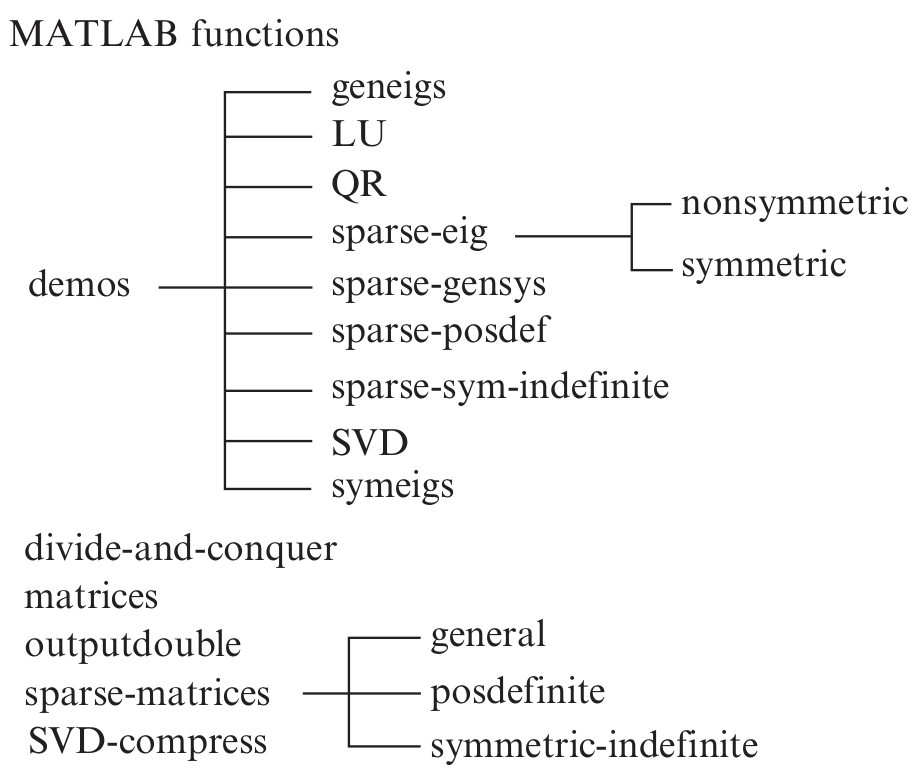
\includegraphics[width=0.6\linewidth]{fig_0_1}
	\caption{NLALIB hierarchy.}
	\label{fig:fig_0_1}
\end{figure}


\subsection*{SUPPLEMENTS}
At \url {http://textbooks.elsevier.com/web/Manuals.aspx?isbn=9780123944351}, the instructor will find supplements that include
the solution to every problem in the book, laboratory exercises that can be used after lectures for more interactive learning, and a complete set of PowerPoint slides. For students, Elsevier provides the Web site \url{http://booksite.elsevier.com/978012394435} that provides students with review questions and solutions. The author also provides the Web site \url{http://ford-book.info} that provides a summary of the book and links to associated Web sites.

\subsection*{ACKNOWLEDGMENTS}
Although I have co-authored a number of books in computer science, this is my first mathematics text. I am indebted to Patrcia Osborn, the acquisitions editor at Elsevier who had faith in the book and ushered it through the acceptance phase. I would also like to thank the reviewers of the book, Jakub Kurzak, Ph.D., Research Director, Innovative Computing Laboratory, University of Tennessee, Rajan Bhatt, Ph.D., research engineer at the University of Iowa Center for Computer Aided Design, and Zhongshan Li, Ph.D., Professor and Graduate Director of Mathematics, Georgia State University. Their comments were helpful and encouraging. I also appreciate the efforts of the editorial project managers, Jill Cetel, Jessica Vaughn, and Paula Callaghan, who were invaluable in helping me through what is a difficult process. I also wish to thank Anusha Sambamoorthy, Project Manager, Book Production, Chennai, Elsevier, for her help with getting the book into print. 

Dr Keith Matthews, Honorary Research Consultant, University of Queensland, gave me permission to use his online textbook, Elementary Linear Algebra, as a starting point for the material in the first six chapters. While I have made many changes to suit the needs of the book, his generosity saved me much time.
I thank the University of the Pacific, School of Engineering and Computer Science, Stockton, California, for providing resources and a sabbatical leave during the development of the book. I also appreciate comments made by engineering graduate students as I used the manuscript in an advanced computation course. Lastly, I am indebted to William Topp, Ph.D., with whom I have coauthored a number of books. He provided encouragement and consolation during the lengthy process of developing the text.

\chapter{Matrices}
\label{chap:chap_1}
\pagenumbering{arabic}
\setcounter{page}{1}

You should be familiar with
\begin{itemize}[noitemsep]
	\item Two- and three-dimensional geometry
	\item Elementary functions 
\end{itemize}

Linear algebra is a branch of mathematics that is used by engineers and applied scientists to design and analyze complex systems. Civil engineers use linear algebra to design and analyze load-bearing structures such as bridges. Mechanical
engineers use linear algebra to design and analyze suspension systems, and electrical engineers use it to design and analyze electrical circuits. Electrical, biomedical, and aerospace engineers use linear algebra to enhance X-rays, tomographs, and
images from space. This introduction is intended to serve as a basis for the study of numerical linear algebra, the study of procedures used on a computer to perform linear algebra computations, most notably matrix operations. As you will see,
there is a big difference between theoretical linear algebra and applying linear algebra on a computer and obtaining reliable results. It is assumed only that the reader has completed one or more calculus courses and has had some exposure to vectors and matrices, although the text provides a review of the basic concepts. It will be helpful but not necessary if the reader has taken a course in discrete mathematics that provided some exposure to mathematical proofs.

 \autoref{sec:sec_1_1} discusses matrix operations, including matrix multiplication and that matrix multiplication obeys many of the familiar laws of arithmetic apart from the commutative law. While matrix multiplication is most often performed on a
computer, it is necessary to understand its definition, fundamental properties, and applications. For instance, a linear system of equations is elegantly expressed in matrix form. This section also introduces the matrix trace operator and the very useful fact that $trace (AB) = trace (BA)$ for square matrices $A$ and $B$. This section concludes with a presentation of basic MATLAB operations for executing these fundamental matrix operations.

A linear transformation is an absolutely critical concept in linear algebra, and  \autoref{sec:sec_1_2} presents the concept and shows how a linear transformation performs a rotation of a figure in the xy-plane or in three-dimensional space. This application
of linear transformations is fundamental to computer graphics. 

 \autoref{sec:sec_1_3} discusses powers of matrices and shows the connection between matrix powers and the number of possible paths between two vertices of a graph. This section also presents the interesting Fibonacci matrix.

\autoref{sec:sec_1_4} introduces the matrix inverse and a number of its properties. It is shown that a linear system has a unique solution when its coefficient matrix has an inverse.

\autoref{sec:sec_1_5} discusses the matrix transpose and this motivates the definition of a symmetric matrix. As we will see in later chapters, symmetric matrices have many applications in engineering and science.

\section[Matrix Arithmetic]{MATRIX ARITHMETIC}
\label{sec:sec_1_1}
A matrix is a rectangular array of numbers with $m$ rows and $n$ columns. The symbol $R^{m \times n}$ denotes the collection of all $m \times n$ matrices whose entries are real numbers. Matrices will usually be denoted by capital letters, and the notation $A = [a_{ij}]$ specifies that the matrix is composed of entries $a_{ij}$ located in the $i$th row and $j$th column of $A$.
A vector is a matrix with either one row or one column; for instance,

\begin{equation*}
	x = 
	\begin{bmatrix}
	1 \\
	-2 \\
	 6\\
	\end{bmatrix}
\end{equation*}

is a column vector, and

\begin{equation*}
y = 
\begin{bmatrix}
6 & -1 & 3\\
\end{bmatrix}
\end{equation*}
is a row vector. The elements of a vector require only one subscript. For the vector $x, x{2} = -4$.

\begin{example}
	The formula $a_{ij} = 1/(i + j)$ for $1 \leq i \leq 3, 1 \leq j \leq 4$ defines a $3 \times 4$ matrix $A = [a_{ij}]$, namely,

	$$ A =
	\begin{bmatrix}
	\frac{1}{2} & \frac{1}{3} & \frac{1}{4} & \frac{1}{5} \\
	\frac{1}{3} & \frac{1}{4} & \frac{1}{5} & \frac{1}{6} \\
	\frac{1}{4} & \frac{1}{5} & \frac{1}{6} & \frac{1}{7}
	\end{bmatrix}
	. $$
	The first column of $A$ is the column vector
	$
	\begin{bmatrix}
		\frac{1}{2} \\ \frac{1}{3} \\ \frac{1}{4}\\
	\end{bmatrix}.
	$
\end{example}

\begin{definition}[Equality of matrices]
	\label{defn:defn_1_1}
	Matrices $A$ and $B$ are said to be equal if they have the same size and their corresponding elements are equal; i.e., $A$ and $B$ have dimension $m \times n$, and $A = [a_{ij}], B = [b{ij}],$ with $a_{ij} = b_{ij}$ for $1 \leq i \leq m, 1 \leq j \leq n.$
\end{definition}

\begin{definition}[Addition of matrices]
	\label{defn:defn_1_2}
	Let $A = [a_{ij}]$ and $B = [b_{ij}]$ be of the same size. Then $A+B$ is the matrix obtained by adding corresponding elements of $A$ and $B$; that is,
	$$A + B = [a_{ij}] + [b_{ij}] = [a_{ij} + b_{ij}].$$
\end{definition}

\begin{definition}[Scalar multiple of a matrix]
	\label{defn:defn_1_3}
	Let $A = [a_{ij}]$ and $t$ be a number ($scalar$). Then $tA$ is the matrix obtained by multiplying all elements of $A$ by $t$; that is,
	$$tA = t[a_{ij}] = [ta_{ij}].$$
\end{definition}

\begin{definition}[Negative of a matrix]
	\label{defn:defn_1_4}
	Let $A = [a_{ij}].$ Then $-A$ is the matrix obtained by replacing the elements of $A$ by their negatives; that is,
	$$-A = -[a_{ij}] = [-a_{ij}].$$
\end{definition}

\begin{definition}[Subtraction of matrices]
	\label{defn:defn_1_5}
	Matrix subtraction is defined for two matrices $A = [a_{ij}]$ and $B = [b_{ij}]$ of the same size, in the usual way; that is,
	$$A - B = [a_{ij}] - [b_{ij}] = [a_{ij} - b_{ij}]. $$
\end{definition}

\begin{definition}[The zero matrix]
	\label{defn:defn_1_6}
	Each $m \times n$ matrix, all of whose elements are zero, is called the zero matrix (of size $m \times n$) and is denoted by the symbol $0$.
\end{definition}


The matrix operations of addition, scalar multiplication, negation and subtraction satisfy the usual laws of arithmetic. (In what follows, $s$ and $t$ are arbitrary scalars and $A, B, C$ are matrices of the same size.)

\begin{enumerate}[label = \textbf{\arabic*. }, noitemsep]
	\item  $(A + B) + C = A + (B + C)$;
	\item  $ A + B = B + A$;
	\item  $0 + A = A$;
	\item  $A + (-A) = 0$;
	\item  $(s + t)A = sA + tA, (s - t)A = sA - tA$;
	\item  $t(A + B) = tA + tB, t(A - B) = tA - tB$;
	\item  $s(tA) = (st)A$;
	\item  $1A = A, 0A = 0, (-1)A = -A$;
	\item  $tA = 0 \Rightarrow t = 0 or A = 0$.
\end{enumerate}

\noindent Other similar properties will be used when needed.

\subsection{Matrix Product}
\label{sec:sec_1_1_1}

\begin{definition}[Matrix product]
	\label{defn:defn_1_7}
	Let $A = [a_{ij}]$ be a matrix of size $m \times p$ and $B = [b_{jk}]$ be a matrix of size $p \times n$ (i.e., the number of columns of $A$ equals the number of rows of $B$). Then $AB$ is the $m \times n$ matrix $C = [c_{ik}]$ whose $(i, j)$th element is defined by the formula
\end{definition}


\begin{figure}
	\centering
	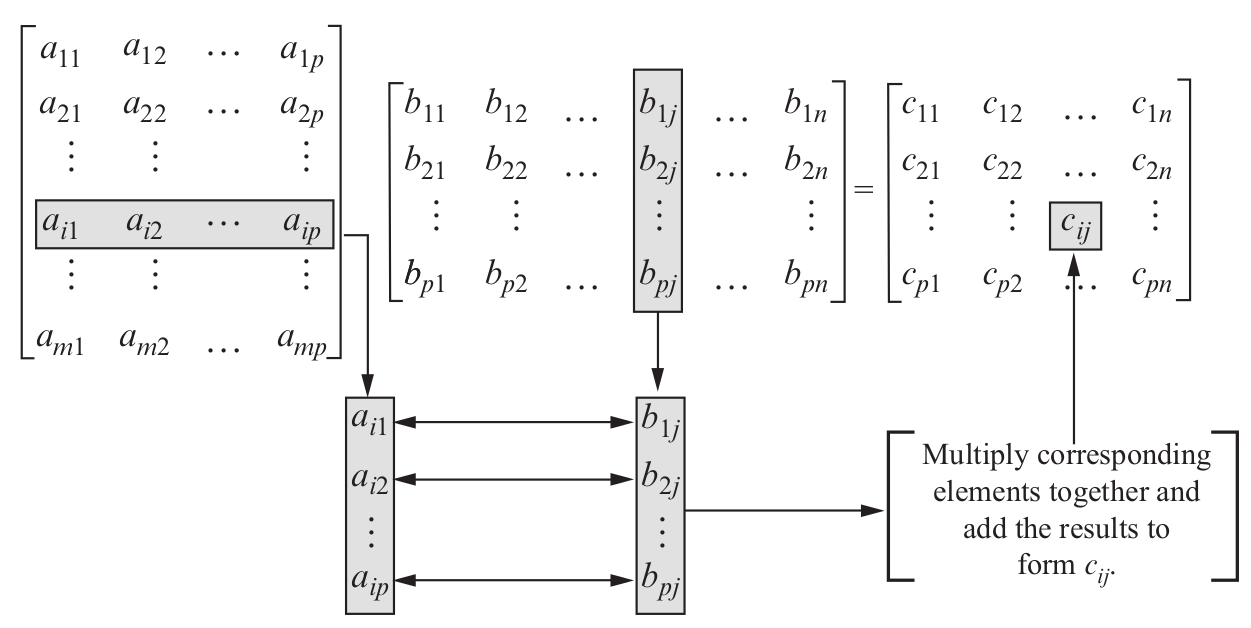
\includegraphics[width=0.7\linewidth]{fig_1_1}
	\caption{Matrix multiplication.}
	\label{fig:fig_1_1}
\end{figure}

$$c_{ij} =  \sum_{k=1}^{p} a_{ik} b_{kj} = a_{i1} b_{1j} + \cdots + a_{ip} b_{pj} .$$

A way to look at this is that $c_{ij}$ is the sum of the products of corresponding elements from row $i$ of $A$ and column $j$ of $B$. For hand computation, fix on row $1$ of $A$. Form the sum of products of corresponding elements from row $1$ of $A$ and column $1$ of $B$, then the sum of products of corresponding elements from row $1$ of $A$ and column $2$ of $B$, and so forth, until forming the sum of the products of corresponding elements of row $1$ of $A$ and column $n$ of $B$. This computes the first row of the product matrix $C$. Now use row $2$ of $A$ in the same fashion to compute the second row of $C$. Continue until you have all $m$ rows of C (\autoref{fig:fig_1_1}).

\begin{example}
	\begin{align}
		\begin{bmatrix}
		1&2\\
		3&4\\
		\end{bmatrix}
		\begin{bmatrix}
		5&6\\
		7&8\\
		\end{bmatrix} &=
		\begin{bmatrix}
		1 \times 5 + 2 \times 7&1 \times 6 + 2 \times 8\\
		3 \times 5 + 4 \times 7&3 \times 6 + 4 \times 8\\
		\end{bmatrix} =
		\begin{bmatrix}
		19 & 22 \\
		43 & 50 \\
		\end{bmatrix}, \nonumber \\
		\begin{bmatrix}
		5&6\\
		7&8\\
		\end{bmatrix}
		\begin{bmatrix}
		1&2\\
		3&4\\
		\end{bmatrix} &=
		\begin{bmatrix}
		23 & 34 \\
		31 & 46 \\
		\end{bmatrix} \neq
		\begin{bmatrix}
		1&2\\
		3&4\\
		\end{bmatrix}
		\begin{bmatrix}
		5&6\\
		7&8\\
		\end{bmatrix}, \nonumber \\
		\begin{bmatrix}
		1\\2\\
		\end{bmatrix}
		\begin{bmatrix}
		3&4\\
		\end{bmatrix} &=
		\begin{bmatrix}
		3&4\\
		6&8\\
		\end{bmatrix}, \nonumber \\
		\begin{bmatrix}
		3 & 4\\
		\end{bmatrix}
		\begin{bmatrix}
		1\\2\\
		\end{bmatrix} &=
		\begin{bmatrix}
		11\\
		\end{bmatrix},	\nonumber \\
		\begin{bmatrix}
		1&-1\\
		1&-1\\
		\end{bmatrix}
		\begin{bmatrix}
		1&-1\\
		1&-1\\
		\end{bmatrix} &=
		\begin{bmatrix}
		0&0\\
		0&0\\
		\end{bmatrix}. \nonumber
	\end{align}
\end{example}

\begin{remark}
	Matrix multiplication is a computationally expensive operation. On a computer, multiplication is a much more time-consuming operation than addition. Consider computing the product of an $m \times  k$ matrix $A$ and a $k \times n$ matrix $B$. The computation of $(AB)_{ij}$ requires calculating $k$ products. This must be done $n$ times to form each row of $AB$, so the computation of a row of $AB$ requires $kn$ multiplications. There are $m$ rows in $AB$, so the total number of multiplications is $m (kn) = mkn$. If $A$ and $B$ are both $n \times n$ matrices, $n^{3}$ multiplications must be performed. For example, if the matrices have dimension $10 \times 10$, the computation of their product requires 1000 multiplications. To multiply two 100 × 100 matrices involves computing 1,000,000 products. A matrix most of whose entries are zero is called sparse. There are faster ways to multiply sparse matrices, and we will deal with these matrices in \autoref{chap:chap_21} and \ref{chap:chap_22}.
\end{remark}

\begin{theorem}
	\label{theo:theo_1_1}
	 Matrix multiplication obeys many of the familiar laws of arithmetic apart from the commutative law.
\begin{enumerate}[label=\textbf{\arabic*}), noitemsep]
	\item $(A B) C=A(B C)$ if $A, B, C$ are $m \times p, p \times k, k \times n$, respectively;
	\item$t(A B)=(t A) B=A(t B), A(-B)=(-A) B=-(A B)$;
	\item $(A+B) C=A C+B C$ if $A$ and $B$ are $m \times n$ and $C$ is $n \times p$;
	\item$D(A+B)=D A+D B$ if $A$ and $B$ are $m \times n$ and $D$ is $p \times m$.
\end{enumerate}
\end{theorem}

We prove the associative law only:

\begin{proof}
	Assume that $A$ is an $m \times p$ matrix, $B$ is a $p \times k$ matrix, and $C$ is a $k \times n$ matrix. Observe that $(A B) C$ and $A(B C)$ are both of size $m \times n$.


	Let $A=\left[a_{i q}\right], B=\left[b_{q l}\right], C=\left[c_{l j}\right]$. Then
	$$
	\begin{aligned}
	((A B) C)_{i j} &=\sum_{q=1}^{k}(A B)_{i q} c_{q j}=\sum_{q=1}^{k}\left(\sum_{l=1}^{p} a_{i l} b_{l q}\right) c_{q j} \\
	&=\sum_{q=1}^{k} \sum_{l=1}^{p} a_{i l} b_{l q} c_{q j}
	\end{aligned}
	$$
	Similarly,
	$$
	(A(B C))_{i j}=\sum_{l=1}^{p} \sum_{q=1}^{k} a_{i l} b_{l q} c_{q j} .
	$$
	However, the double summations are equal. Sums of the form
	$$
	\sum_{q=1}^{k} \sum_{l=1}^{p} d_{l q} \quad \text { and } \quad \sum_{l=1}^{p} \sum_{q=1}^{k} d_{l q}
	$$
	represent the sum of the $k p$ elements of the rectangular array $\left[d_{l q}\right]$, by rows and by columns, respectively. Consequently, $((A B) C)_{i j}=(A(B C))_{i j}$ for $1 \leq i \leq m, 1 \leq j \leq n .$ Hence, $(A B) C=A(B C)$.
	\end{proof}

One of the primary uses of matrix multiplication is formulating a system of equations as a matrix problem. The system of $m$ linear equations in $n$ unknowns
$$
\begin{aligned}
a_{11} x_{1}+a_{12} x_{2}+\cdots+a_{1 n} x_{n}=& b_{1} \\
a_{21} x_{1}+a_{22} x_{2}+\cdots+a_{2 n} x_{n}=& b_{2} \\
\vdots & \\
a_{m 1} x_{1}+a_{m 2} x_{2}+\cdots+a_{m n} x_{n}=&b_{m}
\end{aligned}
$$
is equivalent to a single-matrix equation.
$$
\left[\begin{array}{llll}
a_{11} & a_{12} & \ldots & a_{1 n} \\
a_{21} & a_{22} & \ldots & a_{2 n} \\
\vdots & \vdots & & \vdots \\
a_{m 1} & a_{m 2} & \ldots & a_{m n}
\end{array}\right]\left[\begin{array}{c}
x_{1} \\
x_{2} \\
\vdots \\
x_{n}
\end{array}\right]=\left[\begin{array}{c}
b_{1} \\
b_{2} \\
\vdots \\
b_{m}
\end{array}\right]
$$
that is, $A x=b$, where $A=\left[a_{i j}\right]$ is the coefficient matrix of the system, $x=\left[\begin{array}{l}x_{1} \\ x_{2} \\ \vdots \\ x_{n}\end{array}\right]$ is the vector of unknowns and $b=\left[\begin{array}{l}b_{1} \\ b_{2} \\ \vdots \\ b_{m}\end{array}\right]$ is the vector of constants.

Another useful matrix equation equivalent to the above system of linear equations is
$$
x_{1}\left[\begin{array}{l}
a_{11} \\
a_{21} \\
\vdots \\
a_{m 1}
\end{array}\right]+x_{2}\left[\begin{array}{l}
a_{12} \\
a_{22} \\
\vdots \\
a_{m 2}
\end{array}\right]+\cdots+x_{n}\left[\begin{array}{l}
a_{1 n} \\
a_{2 n} \\
\vdots \\
a_{m n}
\end{array}\right]=\left[\begin{array}{l}
b_{1} \\
b_{2} \\
\vdots \\
b_{m}
\end{array}\right]
$$

We will begin a study of $n \times n$ linear systems in \autoref{chap:chap_2} and continue the study throughout the book. In \autoref{chap:chap_16}, most of the systems we deal with will have dimension $m \times n$, where $m \neq n$.

\begin{example}
The system
$$
\begin{aligned}
x+y+z &=1 \\
x-y+z &=0 \\
3 x+5 y-z &=2
\end{aligned}
$$
is equivalent to the matrix equation
$$
\begin{bmatrix}
1 & 1 & 1 \\
1 & -1 & 1 \\
3 & 5 & -1
\end{bmatrix}\begin{bmatrix}
x \\
y \\
z
\end{bmatrix}=\begin{bmatrix}
1 \\
0 \\
2
\end{bmatrix}
$$
and to the equation
$$
x\begin{bmatrix}
1 \\
1 \\
3
\end{bmatrix}+y\begin{bmatrix}
1 \\
-1 \\
5
\end{bmatrix}+z\begin{bmatrix}
1 \\
1 \\
-1
\end{bmatrix}=\begin{bmatrix}
1 \\
0 \\
2
\end{bmatrix}.
$$
The solution to the system is $\begin{bmatrix}0.0000 \\ 0.5000 \\ 0.5000\end{bmatrix}$:
$$
\begin{aligned}
	 (1) ~0.0000 + (1) 0.5000 + (1)  0.5000=1 \nonumber \\
	 (1) ~0.0000 - (1) 0.5000 +  (1)  0.5000=0  \nonumber \\
	3  ~(0.0000)+5(0.5000)-(1) 0.5000=2
\end{aligned}
$$
\end{example}
\subsection {The Trace}
The trace is a matrix operation that is frequently used in matrix formulas, and it is very simple to compute.

\begin{definition}
	\label{defn:defn_1_8}
	If $A$ is an $n \times n$ matrix, the trace of $A$, written trace $(A)$, is the sum of the diagonal elements; that is,
$$
\operatorname{trace}(A)=a_{11}+a_{22}+\cdots+a_{n n}=\sum_{i=1}^{n} a_{i i}
$$
\end{definition}

\begin{example}If $A=
\begin{bmatrix}
	5 & 8 & 12 & -1 \\
	7 & 4 & -8 & 7 \\
	 0 & 3 & -6 & 5 \\
	 -1 & -9 & 4 & 3
\end{bmatrix}$,
 then trace $(A)=5+4+(-6)+3=6$.
 \end{example}

There are a number of relationships satisfied by trace. For instance, \textsf{trace}$(A+B)$ = \textsf{trace}($A$) + \textsf{trace}($B$).
(\textcolor{blue}{Problem \ref{pro:pro_1_22}} (a)), and \textsf{trace} $(c A)$ = $c$ \textsf{trace} ($A$), where $c$ is a scalar (\textcolor{blue}{Problem \ref{pro:pro_1_22}} (b)) . A more complex relationship is the trace of product of two matrices.

\begin{theorem}
	\label{theo:theo_1_2}
	If $A$ is an $n \times n$ matrix and $B$ is an $n \times n$ matrix, then trace $(A B)=\operatorname{trace}(B A)$.
\end{theorem}


\begin{proof}
	By the definition of matrix multiplication,
	$$
	\operatorname{trace}(A B)=\sum_{i=1}^{n}(A B)_{i i}=\sum_{i=1}^{n}\left(\sum_{k=1}^{n} a_{i k} b_{k i}\right)=\sum_{k=1}^{n}\left(\sum_{i=1}^{n} b_{i k} a_{k i}\right)=\operatorname{trace}(B A)
	$$
\end{proof}

\subsection{MATLAB Examples}
There are numerous examples throughout this book that involve the use of MATLAB. It is fundamental to our use of
MATLAB that you are familiar with \emph{“vectorization.”} When performing vector or matrix operations using the operators “\textasteriskcentered”,
“$/$”, and “\textasciicircum”, it may be necessary to use the dot operator ("."). As stated in the preface, the reader is expected to be familiar
with MATLAB, but it is not necessary to be an expert. \\

\begin{example}\emph{Matrix Operations}
\label{exm:exm_1_5}
The operators +, -, * work as expected in MATLAB, and the command \texttt{trace} computes the trace of a matrix.

\begin{lstlisting}[numbers=none,frame=none]
>> A = [1 5 1;2 -1 6;1 0 3]
A =
		1		5		1
		2		-1	6
		1		0		3
>> B = [2 3 0;3 -1 7;4 8 9]
B =
		2		3		0
		3		-1	7
		4		8		9
>> 5*A -10*B + 3*A*B
ans =
		48 		13 		137
		55 		170		101
		7			1			6
>> trace(A + B)
ans =
		13
>> 7*trace(A + B)
ans =
		91
>> trace(A*B)
ans =
		103
>> trace(B*A)
ans =
		103
>> A.*B
ans =
		2 		15 		0
		6 		1 		42
		4 		0 		27
\end{lstlisting}
\end{example}

\section[Linear Transformations]{LINEAR TRANSFORMATIONS}
\label{sec:sec_1_2}
Throughout this book we will assume that matrices have elements that are real numbers. The real numbers include the integers $(\ldots,-2,-1,0,1,2, \ldots)$, which are a subset of the \emph{rational numbers} $(p / q)$, where $p$ and $q$ are positive integers. $q \neq 0$. The remaining numbers are called \emph{irrational numbers}; for instance, $\pi$ and $e$ are irrational numbers. We will use the symbol \texttt{R} to denote the collection of real numbers. An \emph{$n$ -dimensional column vector} is an $n \times 1$ matrix. The collection of all $n$ -dimensional column vectors is denoted by \texttt{R}$^{n}$.

Every matrix is associated with a type of function called a \emph{linear transformation}.

\begin{definition} [Linear transformation]
	\label{defn:defn_1_9}
	We can associate an $m \times n$ matrix $A$ with the function $T_{A}: R^{n} \rightarrow R^{m}$, defined by $T_{A}(x)=A x$ for all $x \in R^{n} .$ More explicitly, using components, the above function takes the form
$$
\begin{aligned}
y_{1} &=a_{11} x_{1}+a_{12} x_{2}+\cdots+a_{1 n} x_{n} \\
y_{2} &=a_{21} x_{1}+a_{22} x_{2}+\cdots+a_{2 n} x_{n} \\
&\vdots \\
y_{m} &=a_{m 1} x_{1}+a_{m 2} x_{2}+\cdots+a_{m n} x_{n}
\end{aligned}
$$
where $y_{1}, y_{2}, \ldots, y_{m}$ are the components of the column vector $T_{A}(x)$, in other words $y=A x$.

A linear transformation has the property that
$$
T_{A}(s x+t y)=s T_{A}(x)+t T_{A}(y)
$$
for all $s, t \in$ \texttt{R} and all $n$ -dimensional column vectors $x, y .$ This is true because
$$
T_{A}(s x+t y)=A(s x+t y)=s(A x)+t(A y)=s T_{A}(x)+t T_{A}(y)
$$
\end{definition}

\subsection{Rotations}
One well-known example of a linear transformation arises from rotating the $(x, y)$ -plane in two-dimensional Euclidean space counterclockwise about the origin $(0,0)$ through $\theta$ radians. A point $(x, y)$ will be transformed into the point $(\bar{x}, \bar{y}) .$ By referring to \autoref{fig:fig_1_2}, the coordinates of the rotated point can be found using a little trigonometry.
$$
\begin{array}{l}
\bar{x}=d \cos (\theta+\alpha)=d \cos (\theta) \cos (\alpha)-d \sin (\theta) \sin (\alpha)=x \cos (\theta)-y \sin (\theta) \\
\bar{y}=d \sin (\theta+\alpha)=d \sin (\theta) \cos (\alpha)+d \cos (\theta) \sin (\alpha)=x \sin (\theta)+y \cos (\theta)
\end{array}
$$
The equations in matrix form are
$$
R=\begin{bmatrix}
\bar{x} \\
\bar{y}
\end{bmatrix}=
\begin{bmatrix}
\cos \theta & -\sin \theta \\
\sin \theta & \cos \theta
\end{bmatrix}
\begin{bmatrix}
x \\
y
\end{bmatrix}
$$

\begin{example}
	Rotate the line $y=5 x+1$ an angle of $30^{\circ}$ counterclockwise. Graph the original and the rotated line.
\begin{figure}
	\centering
	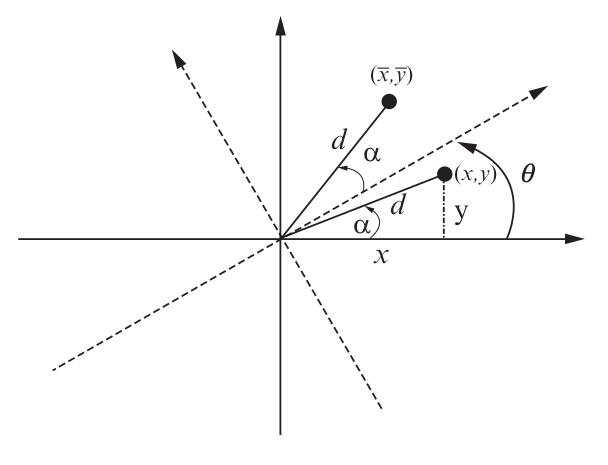
\includegraphics[width=0.7\linewidth]{fig_1_2}
	\caption{Rotating the xy-plane.}
	\label{fig:fig_1_2}
\end{figure}

\begin{figure}
	\centering
	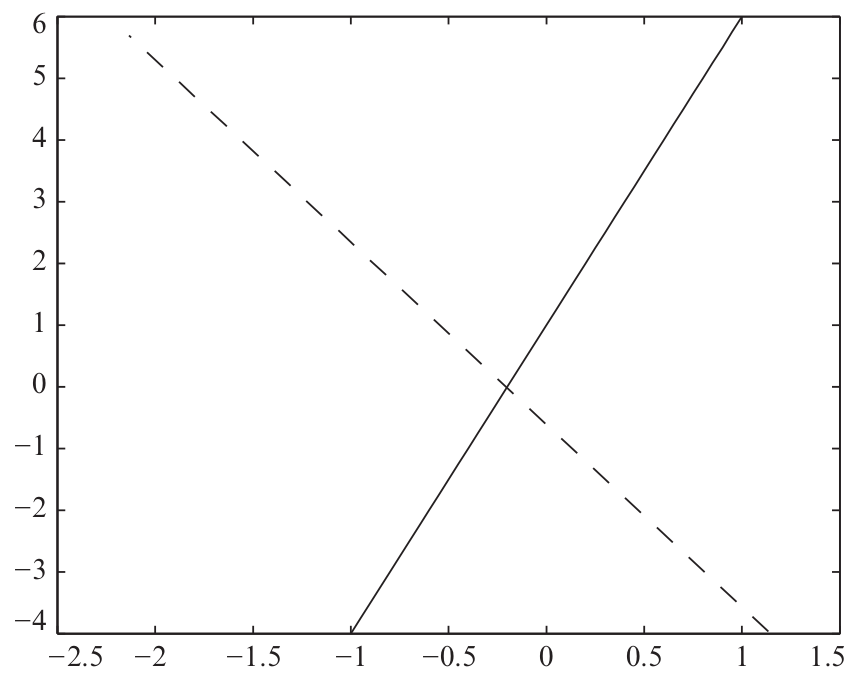
\includegraphics[width=0.7\linewidth]{fig_1_3}
	\caption{Rotated line}
	\label{fig:fig_1_3}
\end{figure}

Since $30^{\circ}$ is $\pi / 6$ radians, the rotation matrix is
$$
\left[\begin{array}{cc}
\cos \frac{\pi}{6} & -\sin \frac{\pi}{6} \\
\sin \frac{\pi}{6} & \cos \frac{\pi}{6}
\end{array}\right]=\left[\begin{array}{cc}
0.866 & -0.5 \\
0.5 & 0.866
\end{array}\right]
$$
Now compute the rotation.
$$
\left[\begin{array}{c}
\bar{x} \\
\bar{y}
\end{array}\right]=\left[\begin{array}{cc}
0.866 & -0.5 \\
0.5 & 0.866
\end{array}\right]\left[\begin{array}{c}
x \\
5 x+1
\end{array}\right]=\left[\begin{array}{c}
-1.634 x-0.5 \\
4.83 x+0.866
\end{array}\right].
$$
Choose two points on the line $y=5 x+1$, say $(0,1)$ and $(1,6)$, apply the transformation to these points, and determine two points on the line.
$$
\begin{bmatrix}
	\overline{x_{1}} \\
	\overline{y_{1}}\\
\end{bmatrix} =
\begin{bmatrix}
-0.5 \\
0.866
\end{bmatrix}\\
\begin{bmatrix}
	\overline{x_{2}} \\
	\overline{y_{2}}
\end{bmatrix} =
\begin{bmatrix}
-2.134 \\
5.696
\end{bmatrix}
$$
 \autoref{fig:fig_1_3} is the graph of the original and the rotated line.
\end{example}

In three-dimensional Euclidean space, the equations
$$
\begin{array}{c}
\bar{x}=x \cos \theta-y \sin \theta, \quad \bar{y}=x \sin \theta+y \cos \theta, \quad \bar{z}=z \\
\bar{x}=x, \quad \bar{y}=y \cos \phi-z \sin \phi, \quad \bar{z}=y \sin \phi+z \cos \phi \\
\bar{x}=x \cos \psi-z \sin \psi, \quad \bar{y}=y, \quad \bar{z}=x \sin \psi+z \cos \psi
\end{array}
$$
correspond to rotations about the positive $z^{-}, x-$, and $y$ -axes, counterclockwise through $\theta, \phi, \psi$ radians, respectively.

The product of two matrices is related to the product of the corresponding linear transformations:

If $A$ is $m \times k$ and $B$ is $k \times n$, the linear transformation $T_{A} T_{B}$ first performs transformation $T_{B}$, and then $T_{A}$. For instance. we might rotate about the $x$ -axis, followed by a rotation about the $z$ -axis. This transformation is in fact equal to the linear transformation $T_{A B}$, since
$$
T_{A} T_{B}(x)=A(B x)=(A B) x=T_{A B}(x)
$$
The following example is useful for producing rotations in three-dimensional animated design (see Ref.  \cite[pp. 97-112]{ref7}).

\begin{figure}
	\centering
	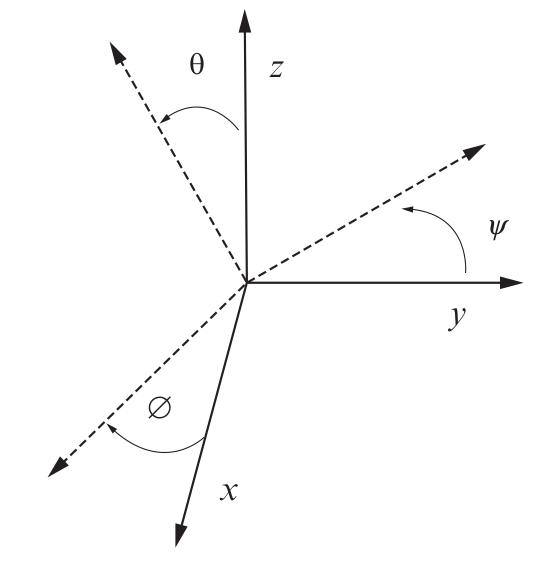
\includegraphics[width=0.4\linewidth]{fig_1_4}
	\caption{Rotate three-dimensional coordinate system}
	\label{fig:fig_1_4}
\end{figure}

\begin{figure}
	\centering
	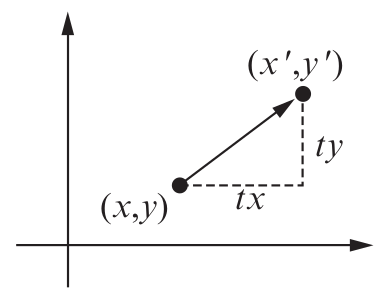
\includegraphics[width=0.4\linewidth]{fig_1_5}
	\caption{Translate a point in two dimensions}
	\label{fig:fig_1_5}
\end{figure}

\begin{example} The linear transformation resulting from successively rotating three-dimensional space about the positive $z, x$, and $y$ -axes, counterclockwise through $\theta, \phi, \psi$ radians, respectively (\autoref{fig:fig_1_4}), is equal to $T_{A B C}$, where
$$
C=\left[\begin{array}{lll}
\cos \theta & -\sin \theta & 0 \\
\sin \theta & \cos \theta & 0 \\
0 & 0 & 1
\end{array}\right], \quad B=\left[\begin{array}{lll}
1 & 0 & 0 \\
0 & \cos \phi & -\sin \phi \\
0 & \sin \phi & \cos \phi
\end{array}\right], \quad A=\left[\begin{array}{lll}
\cos \psi & 0 & -\sin \psi \\
0 & 1 & 0 \\
\sin \psi & 0 & \cos \psi
\end{array}\right]
$$
The matrix $A B C$ is somewhat complex:
$$
\begin{aligned}
A(B C) &=\left[\begin{array}{llll}
\cos \psi & 0 & -\sin \psi \\
0 & 1 & 0 \\
\sin \psi & 0 & \cos \psi
\end{array}\right]\left[\begin{array}{lll}
\cos \theta & -\sin \theta & 0 \\
\cos \phi \sin \theta & \cos \phi \cos \theta & -\sin \phi \\
\sin \phi \sin \theta & \sin \phi \cos \theta & \cos \phi
\end{array}\right] \\
&=\left[\begin{array}{lll}
\cos \psi \cos \theta-\sin \psi \sin \phi \sin \theta & -\cos \psi \sin \theta-\sin \psi \sin \phi \sin \theta & -\sin \psi \cos \phi \\
\cos \phi \sin \theta & \cos \phi \cos \theta & -\sin \phi \\
\sin \psi \cos \theta+\cos \psi \sin \phi \sin \theta & -\sin \psi \sin \theta+\cos \psi \sin \phi \cos \theta & \cos \psi \cos \phi
\end{array}\right]
\end{aligned}
$$
\end{example}

Now consider a new problem. Reposition a point $(x, y)$ along a straight line a distance of $(t x, t y)$, where $t$ is a scalar. The new location of the point is $(x+t x, y+t y)$ (\autoref{fig:fig_1_5}).
To determine a linear transformation, we use a $3 \times 3$ matrix
$$
T=\left[\begin{array}{lll}
1 & 0 & t x \\
0 & 1 & t y \\
0 & 0 & 1
\end{array}\right]
$$
and multiply $T$ by the column vector $\left[\begin{array}{l}x \\ y \\ 1\end{array}\right] .$ Then
$$
\left[\begin{array}{lll}
1 & 0 & t x \\
0 & 1 & t y \\
0 & 0 & 1
\end{array}\right]\left[\begin{array}{l}
x \\
y \\
1
\end{array}\right]=\left[\begin{array}{c}
x+t x \\
y+t y \\
1
\end{array}\right]
$$

In order to combine translation and rotation using matrix multiplication, we need to create a $3 \times 3$ matrix that performs a two-dimensional rotation. Define
$$
R=\left[\begin{array}{ccc}
\cos \theta & -\sin \theta & 0 \\
\sin \theta & \cos \theta & 0 \\
0 & 0 & 1
\end{array}\right]
$$
Now,
$$
\left[\begin{array}{ccc}
\cos \theta & -\sin \theta & 0 \\
\sin \theta & \cos \theta & 0 \\
0 & 0 & 1
\end{array}\right]\left[\begin{array}{l}
x \\
y \\
1
\end{array}\right]=\left[\begin{array}{c}
x \cos \theta-y \sin \theta \\
x \sin \theta+y \cos \theta \\
1
\end{array}\right]
$$
In each case, we can ignore the $z$ component of $1 .$\\

\begin{example} Now we can perform an interesting and practical matrix calculation. Take the line $y=5 x+1$ and rotate it $30^{\circ}$ counterclockwise about the point $(2,11)$.

To solve this problem, first translate the point $(2,11)$ to $(0,0)$, rotate $30^{\circ}$ counterclockwise, and then translate the point from the origin back to $(2,11)$ (\autoref{fig:fig_1_6}).

Here are the matrices involved.

$T_{1}=\left[\begin{array}{ccc}1 & 0 & -2 \\ 0 & 1 & -11 \\ 0 & 0 & 1\end{array}\right] .$ Translate $(2,11)$ to the origin using $t x=-2$ and $t y=-11$\\

$R=\left[\begin{array}{ccc}\cos \frac{\pi}{6} & -\sin \frac{\pi}{6} & 0 \\ \sin \frac{\pi}{6} & \cos \frac{\pi}{6} & 0 \\ 0 & 0 & 1\end{array}\right] .$ Rotate $30^{\circ}$\\

$T_{2}=\left[\begin{array}{lll}1 & 0 & 2 \\ 0 & 1 & 11 \\ 0 & 0 & 1\end{array}\right] .$ Translate back to $(2,11)$ using $t x=2$ and $t y=11 .$\\

Compute the product $F=T_{2} R T_{1}$.
$$
F=\left[\begin{array}{ccc}
0.8660 & -0.5000 & 5.7679 \\
0.5000 & 0.8660 & 0.4737 \\
0 & 0 & 1.0000
\end{array}\right]
$$

\begin{figure}
	\centering
	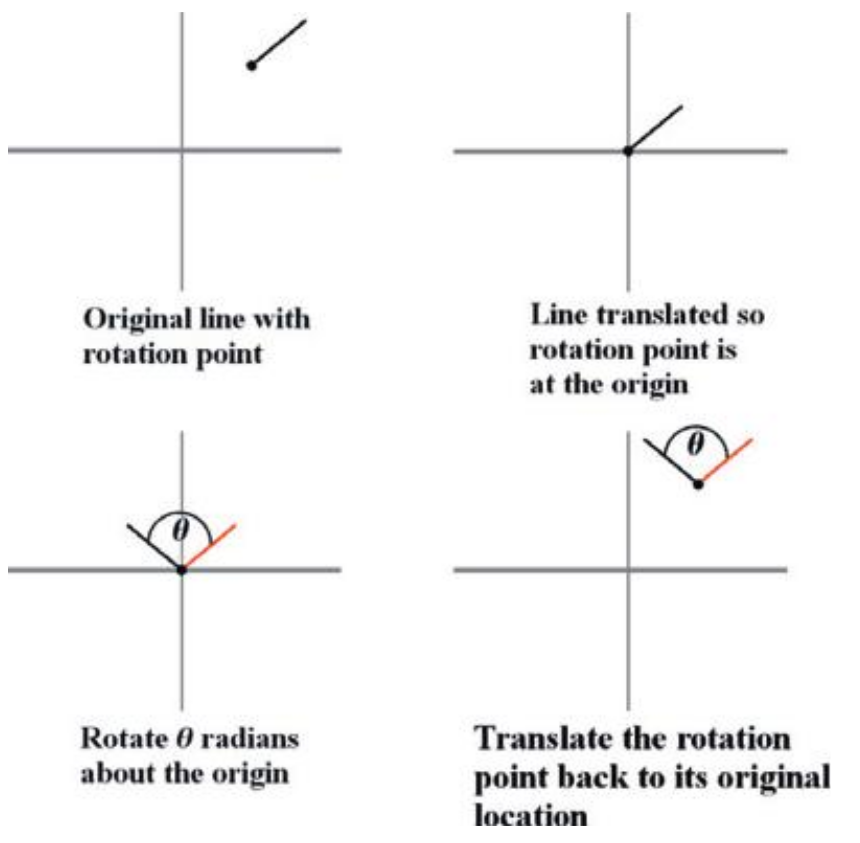
\includegraphics[width=0.7\linewidth]{fig_1_6}
	\caption{Rotate a line about a point.}
	\label{fig:fig_1_6}
\end{figure}

\begin{figure}
	\centering
	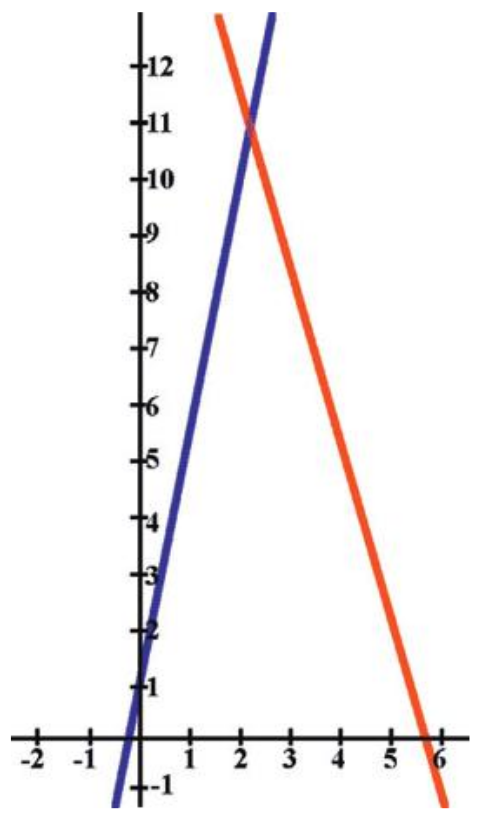
\includegraphics[width=0.4\linewidth]{fig_1_7}
	\caption{ Rotation about an arbitrary point.}
	\label{fig:fig_1_7}
\end{figure}

By computing the two points $F\left[\begin{array}{l}0 \\ 1 \\ 1\end{array}\right]$ and $F\left[\begin{array}{c}2 \\ 11 \\ 1\end{array}\right]$ on the rotated line and using the two point formula for the equation of a line, we obtain the equation $y=-2.9561 x+16.9121$.

\autoref{fig:fig_1_7} is a plot of both the original and the rotated line.
\end{example}

\section[Power of Matrices]{POWERS OF MATRICES}
\label{sec:sec_1_3}

\begin{definition}[The identity matrix]
	\label{defn:defn_1_10}The $n \times n$ matrix $I=\left[\delta_{i j}\right]$, defined by $\delta_{i j}=1$ if $i=j, \delta_{i j}=0$ if $i \neq j$, is called the $n \times n$ identity matrix of order $n$. In other words, the columns of the identity matrix of order $n$ are the vectors
$$
e_{1}=\left[\begin{array}{c}
1 \\
0 \\
\vdots \\
0 \\
0
\end{array}\right], e_{2}=\left[\begin{array}{c}
0 \\
1 \\
\vdots \\
0 \\
0
\end{array}\right], \ldots, e_{n}=\left[\begin{array}{c}
0 \\
0 \\
\vdots \\
0 \\
1
\end{array}\right]
$$
For example, $I=\left[\begin{array}{ll}1 & 0 \\ 0 & 1\end{array}\right]$ and $I=\left[\begin{array}{lll}1 & 0 & 0 \\ 0 & 1 & 0 \\ 0 & 0 & 1\end{array}\right]$. The identity matrix plays a critical role in linear algebra. When any $n \times n$ matrix $A$ is multiplied by the identity matrix, either on the left or the right, the result is $A$. Thus, the identity matrix acts like
1. in the real number system. For example,
$$
\left[\begin{array}{ccc}
2 & 6 & 1 \\
7 & 2 & 9 \\
-1 & 5 & -4
\end{array}\right]\left[\begin{array}{lll}
1 & 0 & 0 \\
0 & 1 & 0 \\
0 & 0 & 1
\end{array}\right]=\left[\begin{array}{ccc}
2(1)+6(0)+1(0) & 2(0)+6(1)+1(0) & 2(0)+6(0)+1(1) \\
7 & 2 & 9 \\
-1 & 5 & -4
\end{array}\right]=\left[\begin{array}{ccc}
2 & 6 & 1 \\
7 & 2 & 9 \\
-1 & 5 & -4
\end{array}\right]
$$\\
\end{definition}

\begin{definition}[kth power of a matrix]
	\label{defn:defn_1_11}
	If $A$ is an $n \times n$ matrix, we define $A^{k}$ as follows: $A^{0}=I$ and $A^{k}=\underbrace{A \times A \times A \cdots A \times A}_{A \text { occurs } k \text { times }}$ for $k \geq 1$.

For example, $A^{4}=A \times A \times A \times A$. Compute from left to right as follows:
$$
A^{2}=A \times A, \quad A^{3}=(A)^{2} \times A, \quad A^{4}=(A)^{3} \times A
$$
\end{definition}

\begin{example} The MATLAB exponentiation operator $^{\wedge}$ applies to matrices.

\begin{lstlisting}[numbers=none,frame=none]
	>> A = [1 1;1 0]
	A =
	1 1
	1 0
	>> A^8
	ans =
	34 21
	21 13
\end{lstlisting}


$A$ is known as the \emph{Fibonacci matrix}, since it generates elements from the famous Fibonacci sequence
$$
0,1,1,2,3,5,8,13,21,34, \ldots
$$\\
\end{example}

\begin{example} Let $A=\left[\begin{array}{cc}7 & 4 \\ -9 & -5\end{array}\right]$. Let's investigate powers of $A$ and see if we can find a formula for $A^{n}$.
$$
\begin{aligned}
A^{2} &=\left[\begin{array}{cc}
7 & 4 \\
-9 & -5
\end{array}\right]\left[\begin{array}{cc}
7 & 4 \\
-9 & -5
\end{array}\right]=\left[\begin{array}{cc}
13 & 8 \\
-18 & -11
\end{array}\right] \\
A^{3} &=\left[\begin{array}{cc}
13 & 8 \\
-18 & -11
\end{array}\right]\left[\begin{array}{cc}
7 & 4 \\
-9 & -5
\end{array}\right]=\left[\begin{array}{cc}
19 & 12 \\
-27 & -17
\end{array}\right], \\
A^{4} &=\left[\begin{array}{cc}
19 & 12 \\
-27 & -17
\end{array}\right]\left[\begin{array}{cc}
7 & 4 \\
-9 & -5
\end{array}\right]=\left[\begin{array}{cc}
25 & 16 \\
-36 & -23
\end{array}\right] \\
A^{5} &=\left[\begin{array}{cc}
25 & 16 \\
-36 & -23
\end{array}\right]\left[\begin{array}{cc}
7 & 4 \\
-9 & -5
\end{array}\right]=\left[\begin{array}{cc}
31 & 20 \\
-45 & -29
\end{array}\right] .
\end{aligned}
$$
The elements in positions $(1,2)$ and $(2,1)$ follow a pattern. The element in position $(1,2)$ is always $4 n$, and the element at position $(2,1)$ is always $-9 n$. The element at $(1,1)$ is $6 n+1$, so we only need the pattern for the entry at $(2,2)$. It is always one $(1)$ more than $-6 n$, so it has the value $1-6 n$. Here is the formula for $A^{n}$
$$
A^{n}=\left[\begin{array}{ll}
1+6 n & 4 n \\
-9 n & 1-6 n
\end{array}\right] \quad \text { if } n \geq 1
$$
This is not a mathematical proof, just an example of pattern recognition. The result can be formally proved using mathematical induction (see \textcolor{blue}{Appendix B}).
\end{example}

Our final example of matrix powers is a result from graph theory. A graph is a set of vertices and connections between them called edges. You have seen many graphs; for example, a map of the interstate highway system is a graph, as is the airline route map at the back of those boring magazines you find on airline flights. Consider the simple graph in \autoref{fig:fig_1_8} A path from one vertex $v$ to another vertex $w$ is a sequence of edges that connect $v$ and $w$. For instance, here are three paths from $A$ to $F: A-B-F, A-B-D-F$, and $A-B-C-E-B-F .$ The length of a path between $v$ and $w$ is the number of edges that must be crossed in moving from one to the other. For instance, in our three paths, the first has length 2, the second has length 3 . and the third has length 5 .

\begin{figure}
	\centering
	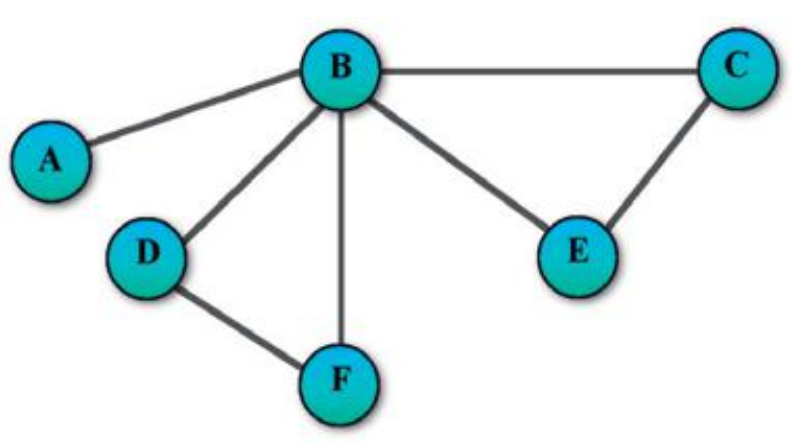
\includegraphics[width=0.4\linewidth]{fig_1_8}
	\caption{Undirected graph.}
	\label{fig:fig_1_8}
\end{figure}

If a graph has $n$ vertices, the \emph{adjacency matrix} of the graph is an $n \times n$ matrix that specifies the location of edges. The concept is best illustrated by displaying the adjacency matrix for six vertex graph, rather than giving a mathematical definition
% % %
$$
\mathrm{Adj}=
\begin{tabular}{r r |r r r r r r|}
& & A & B & C & D & E & F \\
\hline
& A & 0 & 1 & 0 & 0 & 0 & 0 \\
& B & 1 & 0 & 1 & 1 & 1 & 1 \\
& C & 0 & 1 & 0 & 0 & 1 & 0 \\
& D & 0 & 1 & 0 & 0 & 0 & 1 \\
& E & 0 & 1 & 1 & 0 & 0 & 0 \\
& F & 0 & 1 & 0 & 1 & 0 & 0 \\
\end{tabular}
$$

A one (1) occurs in row $A$, column $B$, so there is an edge connecting $A$ and $B$. Similarly, a one is in row $E$, column $C$, so there is an edge connecting $E$ and $C .$ There is no edge between $A$ and $D$, so row $A$, column $D$ contains zero $(0)$

There is a connection between the adjacency matrix of a graph and the number of possible paths between two vertices Clearly, Adj $^{1}$ specifies all the paths of length 1 from one vertex to another (an edge).

\emph{If Adj is the adjacency matrix for a graph, then Adj $^{k}$ defines the number of possible paths of length $k$ between any two vertices.} We will not attempt to prove this, but will use our graph as an example.
$$
\begin{array}{l}
\mathrm{Adj}^{2}=\left[\begin{array}{llllll}
1 & 0 & 1 & 1 & 1 & 1 \\
0 & 5 & 1 & 1 & 1 & 1 \\
1 & 1 & 2 & 1 & 1 & 1 \\
1 & 1 & 1 & 2 & 1 & 1 \\
1 & 1 & 1 & 1 & 2 & 1 \\
1 & 1 & 1 & 1 & 1 & 2
\end{array}\right], \\
\operatorname{Adj}^{3}=\left[\begin{array}{llllll}
0 & 5 & 1 & 1 & 1 & 1 \\
5 & 4 & 6 & 6 & 6 & 6 \\
1 & 6 & 2 & 2 & 3 & 2 \\
1 & 6 & 2 & 2 & 2 & 3 \\
1 & 6 & 3 & 2 & 2 & 2 \\
1 & 6 & 2 & 3 & 2 & 2
\end{array}\right] .
\end{array}
$$
By looking at $\mathrm{Adj}^{2}$, we see that there is one path of length 2 between $C$ and $E, C-B-E$, and two paths of length 2 connecting $E$ to $E(E-C-E, E-B-E) .$ There are five (5) paths of length 3 between $B$ and $A(B-A-B-A, B-D-B-A, B-C-B-A,$, $B-E-B-A, B-F-B-A) .$ Note that if we reverse each path of length three from $B$ to $A$, we have a path that starts at $A$ and ends at $B$. Look carefully at $\mathrm{Adj}, \mathrm{Adj}^{2}$, and $\mathrm{Adj}^{3}$ and notice that the entry at position $(i, j)$ is always the same as the entry at $(j, i) .$ Such a matrix is termed \emph{symmetric}. If you exchange rows and columns, the matrix remains the same. There are many applications of symmetric matrices in science and engineering.

\section[Nonsingular matrices]{NONSINGULAR MATRICES}
\label{sec:sec_1_4}

\begin{definition}[Nonsingular matrix]
	\label{defn:defn_1_12}
	An $n \times n$ matrix $A$ is called \emph{nonsingular} or \emph{invertible} if there exists an $n \times n$ matrix $B$ such that
$$
A B=B A=I
$$
If $A$ does not have an inverse, $A$ is called \emph{singular.}
\end{definition}

A matrix $B$ such that $A B=B A=I$ is called an \emph{inverse} of $A .$ There can only be one inverse, as \autoref{theo:theo_1_3} shows.

\begin{theorem}
	\label{theo:theo_1_3}
	A matrix A can have only one inverse
\end{theorem}

\begin{proof}
	Assume that $A B=I, B A=I$, and $C A=A C=I .$ Then. $C(A B)=(C A) B$, and $C I=I B$, so $C=B$
\end{proof}

When determining if $B$ is the inverse of $A$, it is only necessary to verify $A B=I$ or $B A=I .$ This is important because an procedure that computes the inverse of $A$ need only to verify the product in one direction or the other.\\

\begin{theorem}
\label{theo:theo_1_4}
If $B$ is a matrix such that $B A=I$, then $A B=I .$ Similarly, if $A B=I$, then $B A=I .$
\end{theorem}

\begin{proof}
	Assume that $B A=I$. Then $A B A B=A I B=A B$, and $A B A B-A B=0 .$ Factor out $A B$, and $A B(A B-I)=0 .$ Either $A B=0$ or $A B-I=0 .$ If $A B=0$, then $A B A=0(A)=0 .$ But, $B A=I$, and so it follows that $A=0 .$ The product of any matrix with the zero matrix is the zero matrix, so $B A=I$ is not possible. Thus, $A B-I=0$, or $A B=I .$ The fact that $A B=I$ implies $B A=I$ is handled in the same fashion.
\end{proof}

If we denote the inverse by $A^{-1}$, then
$$
\begin{array}{l}
\left(A^{-1}\right) A=I \\
A\left(A^{-1}\right)=I
\end{array}
$$
and it follows that
$$
\left(A^{-1}\right)^{-1}=A
$$
This says the inverse of $A^{-1}$ is $A$ itself.

The inverse has a number of other properties that play a role in developing results in linear algebra. For instance,
$$
\left(B^{-1} A^{-1}\right)(A B)=B^{-1}\left(A^{-1} A\right) B=B^{-1} I B=B^{-1} B=I
$$
and so
$$
(A B)^{-1}=B^{-1} A^{-1}
$$
By \autoref{theo:theo_1_4}, we do not need to verify that $(A B)\left(B^{-1} A^{-1}\right)=I$.

\begin{remark}
	The above result generalizes to a product of $m$ nonsingular matrices: If $A_{1}, \ldots, A_{m}$ are nonsingular $n \times n$ matrices, then the product $A_{1} \ldots A_{m}$ is also nonsingular. Moreover.
	$$
	\left(A_{1} \ldots A_{m}\right)^{-1}=A_{m}^{-1} \ldots A_{1}^{-1}
	$$
	so the inverse of a product equals the product of the inverses in the reverse order
\end{remark}


\begin{example} If $A$ and $B$ are $n \times n$ matrices satisfying $A^{2}=B^{2}=(A B)^{2}=I$, show that $A B=B A .$
This says that $A, B$, and $A B$ are each their own inverse, or $(A B)^{-1}=A B, B^{-1}=B$, and $A^{-1}=A .$ Now,
$$
A B=(A B)^{-1}=B^{-1} A^{-1}=B A
$$
and so $A B=B A$.
\end{example}

Normally, is it not true that $A B=B A$ for $n \times n$ matrices $A$ and $B .$ For instance.
$$
\left[\begin{array}{cc}
1 & 2 \\
-1 & 5
\end{array}\right]\left[\begin{array}{cc}
6 & 1 \\
-7 & 4
\end{array}\right]=\left[\begin{array}{cc}
-8 & 9 \\
-41 & 19
\end{array}\right],
$$
and
$$
\left[\begin{array}{cc}
6 & 1 \\
-7 & 4
\end{array}\right]\left[\begin{array}{cc}
1 & 2 \\
-1 & 5
\end{array}\right]=\left[\begin{array}{cc}
5 & 17 \\
-11 & 6
\end{array}\right]
$$

\begin{remark}
	We will show how to compute the inverse in \autoref{chap:chap_2}; however, it is computationally expensive. The inverse is primarily a tool for developing other results.
\end{remark}

A matrix having an inverse guarantees that a linear system has a unique solution.


\begin{theorem}
	\label{theo:theo_1_5}
	If the coefficient matrix A of a system of n equations in n unknowns has an inverse, then the system $A x=b$ has the unique solution $x=A^{-1} b$.
\end{theorem}

\begin{proof}
	\begin{enumerate}[label=\textbf{\arabic*}]
\item (Uniqueness) Assume $A x=b$. Then
$$
\begin{aligned}
A^{-1}(A x) &=A^{-1} b, \\
\left(A^{-1} A\right) x &=A^{-1} b, \\
I x &=A^{-1} b, \\
x &=A^{-1} b .
\end{aligned}
$$
\item (Existence) Assume $x=A^{-1} b$. Then
$$
A x=A\left(A^{-1} b\right)=\left(A A^{-1}\right) b=I b=b .
$$
\end{enumerate}
\end{proof}

A linear system $A x=0$ is said to be \emph{homogeneous}. If $A$ is nonsingular, then $x=A^{-1} 0=0$, so the system has only 0 as its solution. It is said to have only the \emph{trivial solution.}

\begin{example} Consider the homogeneous system
$$
\left[\begin{array}{ll}
1 & 3 \\
1 & 2
\end{array}\right] x=0
$$
A simple calculation verifies that $\left[\begin{array}{ll}1 & 3 \\ 1 & 2\end{array}\right]^{-1}=\left[\begin{array}{cc}-2 & 3 \\ 1 & -1\end{array}\right]$, and so
$$
\begin{aligned}
\left[\begin{array}{cc}
-2 & 3 \\
1 & -1
\end{array}\right]\left[\begin{array}{ll}
1 & 3 \\
1 & 2
\end{array}\right] x &=\left[\begin{array}{cc}
-2 & 3 \\
1 & -1
\end{array}\right]\left[\begin{array}{l}
0 \\
0
\end{array}\right] \\
I x &=x=0 .
\end{aligned}
$$
\end{example}

There are some cases where there is an explicit formula for the inverse matrix. In particular, we can demonstrate a formula for the inverse of a $2 \times 2$ matrix subject to a condition. Let $A=\left[\begin{array}{ll}a & b \\ c & d\end{array}\right]$ with $a d-b c \neq 0$ and let $B=(1 /(a d-b c))\left[\begin{array}{cc}d & -b \\ -c & a\end{array}\right] .$ Perform a direct calculation of $A B$
$$
\begin{aligned}
\left[\begin{array}{ll}
a & b \\
c & d
\end{array}\right]\left(\frac{1}{a d-b c}\right)\left[\begin{array}{cc}
d & -b \\
-c & a
\end{array}\right] &=\left(\frac{1}{a d-b c}\right)\left[\begin{array}{ll}
a & b \\
c & d
\end{array}\right]\left[\begin{array}{cc}
d & -b \\
-c & a
\end{array}\right] \\
&=\left(\frac{1}{a d-b c}\right)\left[\begin{array}{ll}
a d-b c & -a b+a b \\
c d-c d & a d-b c
\end{array}\right]=\left[\begin{array}{ll}
1 & 0 \\
0 & 1
\end{array}\right]=I
\end{aligned}
$$

\begin{remark}
	The expression $a d-b c$ is called the determinant of $A$ and is denoted by $\operatorname{det}(A)$. Later we will see that $A$ has an inverse if and only if $\operatorname{det} A \neq 0$.
\end{remark}

The MATLAB function that computes the inverse of an $n \times n$ matrix is  \texttt{inv}. If $A$ is an $n \times n$ matrix, then
\begin{lstlisting}[numbers=none,frame=none]
	>> B = inv(A);
\end{lstlisting}
computes $A^{-1}$.

\begin{example} The following MATLAB statements demonstrate the use of \texttt{inv} and verify that $(AB)^{-1} = B^{-1}A^{-1}$ for two particular matrices

\begin{lstlisting}[numbers=none,frame=none]
	>> format rational;
	>> A = [1 3 -1; 4 1 6; 0 2 3]
	A =
	1	3	-1
	4	1	6
	0	2	3

	>> A_inv = inv(A)
	A_inv =
	9/53	11/53	-19/53
	12/53	-3/53	10/53
	-8/53	2/53	11/53

	>> B = [1 4 0; 3 5 1; 2 -7 8]
	B =
	1  4  0
	3  5  1
	2 -7  8

	>> B_inv = inv(B)
	B_inv =
	-47/41	32/41	-4/41
	22/41	-8/41	1/41
	31/41	-15/41	7/41

	>> inv(A*B)
	ans =
	-7/2173	-621/2173	1169/2173
	94/2173	268/2173	-487/2173
	43/2173	400/2173	-662/2173

	>> B_inv * A_inv
	ans =
	-7/2173	-621/2173	1169/2173
	94/2173	268/2173	-487/2173
	43/2173	400/2173	-662/2173
\end{lstlisting}
\end{example}

\section[The Matrix Transpose and Symmetric Matrices]{THE MATRIX TRANSPOSE AND SYMMETRIC MATRICES}
\label{sec:sec_1_5}
There is another property of a matrix that we will use extensively, the matrix transpose.

\begin{definition}[The transpose of a matrix]
\label{defn:defn_1_13}Let $A$ be on $m \times n$ matrix. Then $A^{\mathrm{T}}$, the transpose of $A$, is the obtained by interchanging the rows and columns of $A$. In other words if $A=\left[a_{i j}\right]$, then $\left(A^{\mathrm{T}}\right)_{i j}=a_{j i}$. Consequently $A^{T}$ is an $n \times m$ matrix.
\end{definition}

For instance, if
$$A=\left[\begin{array}{ccc}1 & 9 & 0 \\ 3 & 7 & 15 \\ 4 & 8 & 1 \\ -7 & 12 & 3\end{array}\right]$$
then
$$A^{\mathrm{T}}=\left[\begin{array}{cccc}1 & 3 & 4 & -7 \\ 9 & 7 & 8 & 12 \\ 0 & 15 & 1 & 3\end{array}\right]$$

\begin{theorem}
	\label{theo:theo_1_6}
	The transpose has the following properties:
\begin{enumerate}[label=\textbf{\arabic*. }, noitemsep]
	\item $(A^{T})^{T} = A$;
	\item$(A \pm B)^{T} = A^{T} \pm B^{T} if~A ~and ~B ~are ~m \times n$;
	\item $(sA)^{T} = sA^{T}~ if ~s ~is ~a ~scalar$;
	\item$(A B)^{T}  = B^{T} A^{T} if ~A ~is ~m \times k ~and ~B ~is ~k \times n$.;
	\item $A ~is ~nonsingular, ~then ~A^{\mathrm{T}} ~is ~also ~nonsingular ~and$ $\left(A^{\mathrm{T}}\right)^{-1}=\left(A^{-1}\right)^{\mathrm{T}}$
	\item $x^{\mathrm{T}} x=x_{1}^{2}+\cdots+x_{n}^{2}$ if $x=\left[x_{1}, \ldots, x_n \right]^T$ is a column vector.
\end{enumerate}
\end{theorem}

\begin{proof}
	We will verify 5 and 6 and leave the remaining properties to exercises.\\
	\textbf{Property 5:} $A^{\mathrm{T}}(\mathrm{A} \left(A^{-1} A\right)^{\mathrm{T}}$ by property 4 . Therefore, $A^{\mathrm{T}}\left(A^{-1}\right)^{T} = I^{T} = I$

	\textbf{Property 6:} $x^{\mathrm{T}} x=\left[\begin{array}{lll}x_{1} & \cdots & x_{n}\end{array}\right]\left[\begin{array}{c}x_{1} \\ \vdots \\ x_{n}\end{array}\right]=x_{1}^{2}+\cdots+x_{n}^{2}$
\end{proof}

There is a frequently  occurring class of matrices defined in terms of the transpose operation.

\begin{definition}[Symmetric matrix]
\label{defn:defn_1_14}A matrix $A$ is symmetric if $A^{\mathrm{T}}=A$. In other words $A$ is square ($m \times n $) and $ a_{ji} = a_{ij}$ $ for all 1 \leq i \leq n, 1 \leq j \leq n$. Another way of looking this is that when the rows and columns are interchanged, the resulting
matrix is A. For instance
$$A=\left[\begin{array}{ll}a & b \\ b & c\end{array}\right]$$
is a general $2 \times 2$ symmetric matrix.
\end{definition}

\begin{example}
 $ A =
\begin{bmatrix}
	1 & 8 & 12 & 3\\
	8 & 5 &  1 & 10\\
	3 & 10 & 9 & 2
\end{bmatrix}$
is a symmetric matrix. Notice row 1 has the same entries as column 1, row 2 has the same entries as column 2, and so forth.
\end{example}

The following proposition proves a property of $A^{\mathrm{T}} A$ that is critical for the computation of what are termed singular values in \autoref{chap:chap_7}.

\begin{proposition}
	If $A$ is an $m \times n$ matrix, then $A^{\mathrm{T}} A$ is a symmetric matrix.
\end{proposition}

\begin{proof}
	$A^{\mathrm{T}} A$ is an $n \times n$ matrix, since $A^{\mathrm{T}}$ has dimension $n \times m$, and $A$ has dimension $m \times n . A^{\mathrm{T}} A$ is symmetric, since
	$$\left(A^{\mathrm{T}} A\right)^{\mathrm{T}}=A^{\mathrm{T}}\left(A^{\mathrm{T}}\right)^{\mathrm{T}}=A^{\mathrm{T}} A$$
\end{proof}
\begin{example} In MATLAB, the transpose operator is '.

\begin{lstlisting}[numbers=none,frame=none]
	>> A = [1 8 -1; 3 -9 15; -1 5 3]
	A =
		1	 8	-1
		3 -9	15
	 -1	 5	 3
	>> A_TA = A'*A
	A_TA =
		 11	 -24	  41
		-24	 170  -128
		 41	-128	 235
	>> A_TA - A_TA'
	ans =
			0	0	0
			0	0	0
			0	0	0
\end{lstlisting}
\end{example}

\section[Chapter Summary]{CHAPTER SUMMARY}
\subsection*{Matrix Arithmetic}
This chapter defines a matrix, introduces matrix notation, and presents matrix operations, including matrix multiplication. To multiply matrices $A$ and $B$, the number of columns of $A$ must equal the number of rows of $B$. It should be emphasized that multiplication of large matrices, most of whose elements are nonzero, is a time-consuming computation. When matrices in applications are very large, they normally consist primarily of zero entries, and are termed sparse. Although matrix multiplication obeys most of the laws of arithmetic, it is not commutative; that is, if $A$ and $B$ are $n \times n$ matrices, $A B$ is rarely equal to $B A$. A vector is a matrix having one row or one column. In this book, we will primarily use column vectors such as
$$
\left[\begin{array}{c}
-1 \\
3 \\
7
\end{array}\right]
$$
The trace of an $n \times n$ matrix is the sum of its diagonal elements $a_{i i}, 1 \leq i \leq n$, or trace $(A)=\sum_{i=1}^{n} a_{i i} .$ The trace occurs in many matrix formulas, and we will encounter it in later chapters. It is important to note that even though $A B \neq B A$ in general, in fact trace $(\mathrm{AB})=\operatorname{trace}(\mathrm{BA})$
A primary topic in this book is the solution of linear systems of equations, and we write them using matrix notation; for instance, the system
$$
\begin{aligned}
x_{1}-x_{2}+5 x_{3} &=1 \\
-2 x_{1}+4 x_{2}+x_{3} &=0 \\
7 x_{1}-2 x_{2}-6 x_{3} &=8
\end{aligned}
$$
using matrix notation is
$$
\left[\begin{array}{ccc}
1 & -1 & 5 \\
-2 & 4 & 1 \\
7 & -2 & -6
\end{array}\right]\left[\begin{array}{l}
x_{1} \\
x_{2} \\
x_{3}
\end{array}\right]=\left[\begin{array}{l}
1 \\
0 \\
8
\end{array}\right]
$$
\subsection*{Linear Transformations}
If $A$ is an $m \times n$ matrix, a linear transformation is a mapping from $\mathsf{R}^{n}$ to $R^{m}$ defined by $y=A x .$ We will deal with linear transformations throughout the remainder of this book. An excellent example is a two-dimensional linear transformation of the form
$$
y=\left[\begin{array}{cc}
\cos \theta & -\sin \theta \\
\sin \theta & \cos \theta
\end{array}\right]\left[\begin{array}{l}
x_{1} \\
x_{2}
\end{array}\right]
$$
that rotates the vector $\left[\begin{array}{l}x_{1} \\ x_{2}\end{array}\right]$ counter clockwise through angle $\theta .$ Such linear transformations perform rotation, displacement, and scaling of objects in computer graphics.

\subsection*{Powers of Matrices}
There are numerous applications of matrix powers, $A^{k}, k \geq 0 .$ Given an undirected graph, powers of the adjacency matrix provide a count of the number of paths between any two vertices.
We will see in \autoref{chap:chap_21}  and \ref{chap:chap_22} that
a sequence of the form $A x_{0}, A^{2} x_{0}, \ldots, A^{k-1} x_{0}$  forms the basis for series of important methods that solve linear systems and compute eigenvalues of large, sparse matrices.
We will discuss solving linear systems in \autoref{chap:chap_2} and eigenvalues in \autoref{chap:chap_5}.

\subsection*{Nonsingular Matrices}
The inverse of a matrix is of great theoretical importance in linear algebra. An $n \times n$ matrix $A$ has inverse $A^{-1}$ if
$$A^{-1} A=A A^{-1}=I$$,
where $I$ is the identity matrix
$$
\left[\begin{array}{ccccc}
1 & 0 & \ldots & \ldots & 0 \\
0 & 1 & 0 & \ldots & 0 \\
0 & 0 & \ddots & \ldots & 0 \\
\vdots & \vdots & \ddots & 1 & \vdots \\
0 & 0 & \ldots & 0 & 1
\end{array}\right]
$$
When it exists, the inverse is unique, and the matrix is termed nonsingular. Not all matrices have an inverse, and such matrices are said to be singular. A linear system $A x=b$ has a unique solution $x=A^{-1} b$ when $A$ is nonsingular. A very important result is that a homogeneous system of the form $A x=0$ has only the solution $x=0$ if $A$ is nonsingular.

\subsection*{The Matrix Transpose and Symmetric Matrices}
The transpose of an $m \times n$ matrix $A$, named $A^{\mathrm{T}}$, is the $n \times m$ matrix obtained by exchanging the rows and columns of $A$. Theorem 1.6 lists properties of the transpose.

An important class of matrices are the symmetric matrices. A square matrix $A$ is symmetric if $A^{\mathrm{T}}=A$, and this means that $a_{i j}=a_{j i}, 1 \leq i, j \leq n .$ Many problems in engineering and science involve symmetric matrices, and entire sections of this book deal with them. As you will see, when a problem involves a symmetric matrix, this normally leads to a faster and more accurate solution.

It is of the utmost importance that you remember the relationship $(A B)^{\mathrm{T}}=B^{\mathrm{T}} A^{\mathrm{T}}$, as we will use it again and again throughout this book. Here is an interesting fact we will use beginning in \autoref{chap:chap_7} If $A$ is any $m \times n$ matrix, then $A^{\mathrm{T}} A$ is symmetric, since
$$
\left(A^{\mathrm{T}} A\right)^{\mathrm{T}}=A^{\mathrm{T}}\left(A^{\mathrm{T}}\right)^{\mathrm{T}}=A^{\mathrm{T}} A
$$

\section[Problems]{PROBLEMS}
\begin{enumerate}[label=\textbf{1.\arabic*}]
	\item For
$$
A=\left[\begin{array}{lll}
1 & 8 & -1 \\
0 & 6 & -7 \\
2 & 4 & 12
\end{array}\right], \quad 	B=\left[\begin{array}{ccc}
6 & -1 & 25 \\
14 & -6 & 0 \\
-9 & 15 & 25
\end{array}\right]
$$
compute the following:
	\begin{enumerate}[label = \textbf{\alph*.}]
		\item $A-B$
		\item $8 A$
		\item $5 A+7 B$
	\end{enumerate}

\item Using the matrices $A$ and $B$ from Problem $1.1$, compute $A B .$ Do not use a computer program. Do it with pencil and paper.

\item Let $A, B, C, D$ be matrices defined by
$$
\begin{array}{c}
A=\left[\begin{array}{cc}
3 & 0 \\
-1 & 2 \\
1 & 1
\end{array}\right], \quad  B=\left[\begin{array}{ccc}
1 & 5 & 2 \\
-1 & 1 & 0 \\
-4 & 1 & 3
\end{array}\right] \\
C=\left[\begin{array}{cc}
-3 & -1 \\
2 & 1 \\
4 & 3
\end{array}\right], \quad D=\left[\begin{array}{cc}
4 & -1 \\
2 & 0
\end{array}\right] .
\end{array}
$$

Which of the following matrices are defined? Compute those matrices which are defined.
$$
A+B, A+C, A B, B A, C D, D C, D^{2}
$$

\item  Let $A=\left[\begin{array}{ccc}-1 & 0 & 1 \\ 0 & 1 & 1\end{array}\right]$. Show that if $B$ is a $3 \times 2$ matrix such that $A B=I$, then
$$
B=\left[\begin{array}{ll}
a & b \\
-a-1 & 1-b \\
a+1 & b
\end{array}\right]
$$
for suitable numbers $a$ and $b$. Use the associative law to show that $(B A)^{2} B=B$.

\item If $A=\left[\begin{array}{ll}a & b \\ c & d\end{array}\right]$, show that $A^{2}-(a+d) A+(a d-b c) I_{2}=0$

\item A square matrix $D=\left[d_{i j}\right]$ is called \emph{diagonal} if $d_{i j}=0$ for $i \neq j$; that is the \emph{off-diagonal} elements are zero. Show that premultiplication of a matrix $A$ by a diagonal matrix $D$ results in matrix $D A$ whose rows are the rows of $A$ multiplied by the respective diagonal elements of $D$.

\item Write the following linear algebraic system in matrix form.
$$
\begin{array}{r}
5 x_{1}+6 x_{2}-x_{3}+2 x_{4}=1 \\
-x_{1}+2 x_{2}+x_{3}-9 x_{4}=8 \\
2 x_{1}-x_{3}=-3 \\
3 x_{2}+28 x_{3}-2 x_{4}=0
\end{array}
$$

\item Write this matrix equation as a system of equations.
$$
\left[\begin{array}{ccc}
1 & 0 & 9 \\
-8 & 3 & 45 \\
12 & -6 & 55
\end{array}\right] x=\left[\begin{array}{l}
1 \\
0 \\
1
\end{array}\right]
$$


\item Define the linear transformation $T_{A}: \mathsf{R}^{5} \rightarrow \mathsf{R}^{5}$ using the matrix
\label{pro:pro_1_9}
$$
A=\left[\begin{array}{llllc}
1 & 7 & 0 & 0 & 0 \\
4 & 5 & 8 & 0 & 0 \\
0 & 6 & 1 & 1 & 0 \\
0 & 0 & 7 & 3 & -9 \\
0 & 0 & 0 & 1 & 2
\end{array}\right]
$$
$A$ is termed a tridiagonal matrix, since the only non-zero entries are along the main diagonal, the diagonal below, and the diagonal above.

	\begin{enumerate}[label = \textbf{\alph*.}]
		\item Compute $A\left[\begin{array}{c}0 \\ 1 \\ -1 \\ 3 \\ 2\end{array}\right] .$
		\item Compute $A\left[\begin{array}{l}6 \\ 0 \\ 1 \\ 3 \\ 0\end{array}\right] .$
		\item Compute the general product
$$
\left[\begin{array}{cccc}
a_{11} & a_{12} & 0 & 0 \\
a_{21} & a_{22} & a_{23} & 0 \\
0 & a_{32} & a_{33} & a_{34} \\
0 & 0 & a_{43} & a_{44}
\end{array}\right]\left[\begin{array}{c}
x_{1} \\
x_{2} \\
x_{3} \\
x_{4}
\end{array}\right]
$$
		\item Propose a formula for the product $y=A x$ of an $n \times n$ tridiagonal matrix $A$ and an $n \times 1$ column vector $x$. Use the result of part (c) to help you formulate your answer.
	\end{enumerate}

\item Rotate the line $y=-x+330^{\circ}$ counterclockwise about the origin, and graph the two lines on the same set of axes.

\item Rotate the line $y=-x+360^{\circ}$ counterclockwise about the point $(4,-1)$, and graph the two lines on the same set of axes.

\item Let $A=\left[\begin{array}{cc}1 & 4 \\ -3 & 1\end{array}\right]$. Show that $A$ is nonsingular by verifying that
$$
A^{-1}=\left[\begin{array}{cc}
\frac{1}{13} & -\frac{4}{13} \\
\frac{3}{13} & \frac{1}{13}
\end{array}\right]
$$

\item Let $A=\left[\begin{array}{ll}1 & 3 \\ 2 & 0\end{array}\right]$

	\begin{enumerate}[label = \textbf{\alph*.}]
		\item Find the inverse of the matrix
		\item Use $A^{-1}$ to solve the system
		$$
		\begin{array}{r}
		x_{1}+3 x_{2}=6 \\
		2 x_{1}-9 x_{2}=1
		\end{array}
		$$
	\end{enumerate}

\item If $A=\left[\begin{array}{cc}1 & 4 \\ -3 & 1\end{array}\right]$
	\begin{enumerate}[label = \textbf{\alph*.}]
		\item Verify that $A^{2}-2 A+13 I=0$
		\item Show that $A^{-1}=-\frac{1}{13}(A-2 I)$
	\end{enumerate}

\item Let $A=\left[\begin{array}{ccc}1 & 1 & -1 \\ 0 & 0 & 1 \\ 2 & 1 & 2\end{array}\right]$. Verify that $A^{3}=3 A^{2}-3 A+I .$

\item Let $A$ be an $n \times n$ matrix.

	\begin{enumerate}[label = \textbf{\alph*.}]
		\item If $A^{2}=0$, prove that $A$ is singular. Start by assuming $A^{-1}$ exists. Compute $A^{-1}(A)^{2}$ and deduce that $A$ must be singular.
		\item If $A^{2}=A$ and $A \neq I$, prove that $A$ is singular. Use the same logic as in part (a).
	\end{enumerate}

\item If $X=\left[\begin{array}{ll}1 & 2 \\ 3 & 4 \\ 5 & 6\end{array}\right]$ and $Y=\left[\begin{array}{c}1 \\ 3 \\ 4\end{array}\right]$, find $X X^{\mathrm{T}}, X^{\mathrm{T}} X, Y Y^{\mathrm{T}}, Y^{\mathrm{T}} Y$

\item For matrices $A$ and $B$, show that $(A B)^{\mathrm{T}}=B^{\mathrm{T}} A^{\mathrm{T}}$.
$$
A=\left[\begin{array}{ccc}
1 & 4 & -1 \\
0 & 7 & 1 \\
1 & 7 & 2
\end{array}\right], \quad
B=\left[\begin{array}{ccc}
1 & 2 & 6 \\
1 & -7 & 3 \\
0 & 1 & 2
\end{array}\right]
$$

\item If $A$ is a symmetric $n \times n$ matrix and $B$ is $n \times m$, prove that $B^{\mathrm{T}} A B$ is a symmetric $m \times m$ matrix.

\item Show that $A=\left[\begin{array}{lll}1 & 0 & 0 \\ 0 & 0 & 1 \\ 0 & 1 & 0\end{array}\right]$ is its own inverse.

\item It is not usually the case for $n \times n$ matrices $A$ and $B$ that $A B=B A$. For instance,
$$
A=\left[\begin{array}{ll}
1 & 2 \\
0 & 3
\end{array}\right], \quad B=\left[\begin{array}{ll}
7 & 3 \\
1 & 8
\end{array}\right], \quad A B=\left[\begin{array}{ll}
9 & 19 \\
3 & 24
\end{array}\right], \quad B A=\left[\begin{array}{ll}
7 & 23 \\
1 & 26
\end{array}\right]
$$
Let $A$ and $B$ be $n \times n$ diagonal matrices:
$$
A=\left[\begin{array}{cccc}
a_{11} & 0 & \cdots & 0 \\
0 & a_{22} & \cdots & 0 \\
\vdots & \vdots & \ddots & \vdots \\
0 & 0 & \cdots & a_{n n}
\end{array}\right], \quad
B=\left[\begin{array}{cccc}
b_{11} & 0 & \cdots & 0 \\
0 & b_{22} & \cdots & 0 \\
\vdots & \vdots & \ddots & \vdots \\
0 & 0 & \cdots & b_{n n}
\end{array}\right]
$$
Show that $A B=B A$.

\item Prove the following formulas are satisfied by the trace matrix operator.
\label{pro:pro_1_22}

	\begin{enumerate}[label = \textbf{\alph*.}]
		\item  $\operatorname{trace}(A+B)=\operatorname{trace}(A)+\operatorname{trace}(B)$
		\item trace $(c A)=\mathrm{c}$ trace $(A)$, where $c$ is a scalar.
	\end{enumerate}

\item For an arbitrary $n \times 1$ column vector and an $n \times n$ matrix A, show that $x^{\mathrm{T}} A x$ is a real number. This is called a \emph{quadratic form.} For $x=\left[\begin{array}{lll}1 & 3 & 9\end{array}\right]^{\mathrm{T}}$, compute $x^{\mathrm{T}} A x$ for the matrix
$$
A=\left[\begin{array}{ccc}
1 & -8 & 3 \\
4 & 0 & -1 \\
3 & 5 & 7
\end{array}\right]
$$

\item Prove the following properties of the matrix transpose operator.

	\begin{enumerate}[label = \textbf{\alph*.}]
		\item $\left(A^{\mathrm{T}}\right)^{\mathrm{T}}=A .$
		\item $(A \pm B)^{\mathrm{T}}=A^{\mathrm{T}} \pm B^{\mathrm{T}}$ if $A$ and $B$ are $m \times n .$
		\item $(s A)^{\mathrm{T}}=s A^{\mathrm{T}}$ if $s$ is a scalar.
	\end{enumerate}

\item Prove that $(A B)^{\mathrm{T}}=B^{\mathrm{T}} A^{\mathrm{T}}$ if $A$ is $m \times n$ and $B$ is $n \times p .$ Hint: Use the definition of matrix multiplication and the fact that taking the transpose means element $a_{i j}$ of $A$ is the element at row $j$, column $i$ of $A^{\mathrm{T}}$

\end{enumerate}

\subsection{MATLAB Problems}

\begin{enumerate}[label=\textbf{1.\arabic*}]
\addtocounter{enumi}{25}

\item For this exercise, use the MATLAB command \texttt{format rational} so the computations are done using rational arithmetic. Find the inverse of matrices $A$ and $B$.
$$
A=\left[\begin{array}{ccc}
1 & 4 & 1 \\
1 & 3 & 2 \\
-1 & 2 & 7
\end{array}\right], \quad B=\left[\begin{array}{ccc}
1 & 0 & 1 \\
2 & 5 & 12 \\
-9 & 1 & 1
\end{array}\right]
$$
Verify that $(A B)^{-1}=B^{-1} A^{-1}$.

\item Use MATLAB to find the inverse of the matrix $A=\left[\begin{array}{cccc}1 & 3 & -1 & -9 \\ 0 & 3 & 0 & 1 \\ 12 & 8 & -11 & 0 \\ 2 & 1 & 5 & 3\end{array}\right]$.


\item The $n \times n$ Hilbert matrices are defined by $H(i, j)=1 /(i+j-1), 1 \leq i, j \leq n .$ For instance, here is the $5 \times 5$ Hilbert matrix.
\label{pro:pro_1_28}
$$
H=\left[\begin{array}{ccccc}
1 & \frac{1}{2} & \frac{1}{3} & \frac{1}{4} & \frac{1}{5} \\
\frac{1}{2} & \frac{1}{3} & \frac{1}{4} & \frac{1}{5} & \frac{1}{6} \\
\frac{1}{3} & \frac{1}{4} & \frac{1}{5} & \frac{1}{6} & \frac{1}{7} \\
\frac{1}{4} & \frac{1}{5} & \frac{1}{6} & \frac{1}{7} & \frac{1}{8} \\
\frac{1}{5} & \frac{1}{6} & \frac{1}{7} & \frac{1}{8} & \frac{1}{9}
\end{array}\right]
$$
Systems of the form $H x=b$, where $H$ is a Hilbert matrix are notoriously difficult to solve because they are illconditioned. This means that a solution can change widely with only a small change in the elements of $b$ or $H .$ \autoref{chap:chap_10} discusses ill-conditioned matrices. The MATLAB command $h i]$ b builds an $n \times n$ Hilbert matrix. For instance to find the $6 \times 6$ Hilbert matrix, execute
	\begin{lstlisting}[numbers=none,frame=none]
	>> H = hilb(6);
	\end{lstlisting}

	\begin{enumerate}[label = \textbf{\alph*.}]
	\item The command
	\begin{lstlisting}[numbers=none,frame=none]
	format shortg
	\end{lstlisting}
	causes output of the best of fixed or floating point format with 5 digits. Using this format, compute the inverse of the $6 \times 6$ Hilbert matrix. What makes you suspicious that it is ill-conditioned?
	\item The exact inverse of any Hilbert matrix consists entirely of integer entries. Using the Symbolic Toolbox will provide an exact answer. If your MATLAB distribution has this software, use the help system to determine how to use the commands \texttt{syms} and \texttt{sym}. Determine the exact value of $H^{-}$
	\end{enumerate}

\item
	\begin{enumerate}[label = \textbf{\alph*.}]
	\item Write a MATLAB \texttt{function t = tr(A)} that computes the trace of matrix $A$. Test to make sure $A$ is a square matrix.
	\item Use \texttt{tr} to compute the trace for the matrix of \textcolor{blue}{Problem \ref{pro:pro_1_9}} and the Hilbert matrix of order 15 (\textcolor{blue}{Problem \ref{pro:pro_1_28}}). Verify your result by using the MATLAB command \texttt{trace}.
	\end{enumerate}

\item This problem uses the result of \textcolor{blue}{Problem \ref{pro:pro_1_9}}(d).
	\begin{enumerate}[label = \textbf{\alph*.}]
		\item Write a MATLAB \texttt{function y = triprod(A,x)} that forms the product of an $n \times  n$ tridiagonal matrix $A$ with an $n \times 1$ column vector $x$.
		\item Test the function using the matrix and vectors specified in \textcolor{blue}{Problem \ref{pro:pro_1_9}}, parts (a), and (b).
	\end{enumerate}
\end{enumerate}

\clearpage

\end{document} 
